\documentclass[11pt]{article}
\usepackage[preprint]{acl}
\usepackage{times}
\usepackage{latexsym}
\usepackage[T1]{fontenc}
\usepackage[utf8]{inputenc}
\usepackage{microtype}
\usepackage{inconsolata}
\usepackage{graphicx}
\usepackage{booktabs}
\usepackage{multirow}
\usepackage{amsmath}

\title{SMRITI: An Evidence-Aware, Contradiction-Constrained Knowledge Graph \\ Architecture for Heterogeneous Notes}

\author{Abhijnan B C \\
  \texttt{p9713889@gmail.com} \\}

\begin{document}
\maketitle

\begin{abstract}
We present SMRITI, a system that converts unstructured personal note
vaults into a reliability-scored, contradiction-aware knowledge graph by
combining claim extraction, embedding-retrieval candidate generation,
NLI-based relationship classification, signed-graph contradiction
partitioning, and multi-signal evidence fusion. An earlier version of this
system reported impressive-looking self-evaluation numbers that turned out,
on inspection, to be structural proxies rather than semantic evaluation
(e.g.\ treating claim ``precision'' as the fraction of extracted claims
that are simply non-empty) and a contradiction classifier whose measured
precision was 3.2\%. Rather than polish those numbers, we rebuilt the
evaluation layer and then rebuilt the algorithm the old evaluation was
hiding problems in. This paper reports that reconstruction: (i) we
deleted every fabricated metric from the system's self-certification layer
and replaced it with a frozen, five-claim research registry in which a
claim without real supporting evidence is honestly reported as
\emph{not evaluable}, never defaulted to a passing score; (ii) we found and
fixed the root algorithmic cause of the 3.2\% contradiction precision --- a
resolver that checked a candidate relationship against only one alternative
class instead of requiring it to be the genuine arg-max among
support/contradiction/neutral scores --- together with a lightweight topical-
relatedness gate that blocks contradiction verdicts between claims sharing
no detectable vocabulary; (iii) we built SMRITI-Controlled, a small corpus
of claim pairs whose relationship label is a fact about how the corpus was
constructed (numeric facts, explicit negation, named-entity attribution),
requiring no annotation of any kind, on which the fixed classifier achieves
100\% precision on every retrieved contradiction pair across six distinct
contradiction categories; (iv) we added metamorphic reliability tests and
an exact audit-trail reconstruction test, both requiring zero external
ground truth; and (v) we re-ran the disclosed LLM-derived reference
annotation from scratch against the corrected system, which discloses
that the fix's benefit does not transfer to SMRITI-Reference's real,
argumentative prose: CONTRADICTS precision there is 4.6\%, statistically
no better than the pre-fix 3.2\%, because most of that corpus's genuine
disagreement is rhetorical rather than propositional, and an
off-the-shelf entailment model does not recognize rhetoric as
contradiction regardless of how faithfully the resolver reports its
verdict. We report all of this, including what still does not work, with
the same discipline we applied to finding what was broken.
\end{abstract}

\section{Introduction}
\label{sec:intro}

Personal knowledge management tools increasingly promise to turn scattered
notes into structured knowledge, but most either (a) perform simple
retrieval/search over notes without any semantic modeling of what a note
\emph{asserts}, or (b) apply a single NLP component (entailment, embedding
similarity, entity linking) in isolation, without addressing what happens
when a user's notes \emph{disagree with themselves} over time. SMRITI
treats this as a first-class problem: it extracts discrete claims,
retrieves semantically related pairs, classifies their relationship, keeps
contradicting claims structurally apart in the resulting knowledge graph,
and fuses multiple evidence signals into a single, auditable reliability
score per claim.

\paragraph{This paper is a correction, not a showcase.} A first version of
this work reported self-certification numbers that looked strong but were
not measuring what they claimed to measure, and a real empirical evaluation
that exposed a genuinely broken contradiction classifier (3.2\% precision).
Confronted with that gap, the temptation is to write around it. We did the
opposite: we treated the gap itself as the research problem. Concretely,
we ask five research questions, each answered by a specific piece of new
evidence in this paper, none of it requiring a human annotation budget we
did not have:

\begin{description}
  \item[RQ1] Can a rule-based assertion classifier, added ahead of claim
    construction, materially improve the semantic validity of extracted
    claims without any model training? (\S\ref{sec:system}, \S\ref{sec:results})
  \item[RQ2] Is SMRITI's originally near-zero contradiction precision an
    algorithmic bug or an irreducible property of using an off-the-shelf
    NLI model --- and if a bug, can it be fixed without a new model?
    (\S\ref{sec:system}, \S\ref{sec:controlled}, \S\ref{sec:results})
  \item[RQ3] Does the fix generalize, or does it only help on the specific
    corpus that exposed the original problem?
    (\S\ref{sec:controlled}, \S\ref{sec:results})
  \item[RQ4] Does evidence-aware reliability fusion behave in the direction
    its own design requires under controlled perturbations, and is every
    reported score exactly reconstructible from its own audit trail?
    (\S\ref{sec:metamorphic})
  \item[RQ5] What, honestly, does this evaluation still not establish, and
    what would? (\S\ref{sec:limitations})
\end{description}

\paragraph{Contributions.}
\begin{itemize}
  \item \textbf{A scientific-validity cleanup} of the system's self-
    certification layer: every fabricated metric (a hard-coded
    ``generalization confidence'' of 50, a ``statistical support'' score
    that rewarded merely registering more experiments, a contradiction-
    graph quality metric with no independent verification) is deleted, not
    patched, and replaced by a frozen five-claim registry (RC1--RC5) with
    an explicit \texttt{NOT\_EVALUABLE} status for anything the system
    cannot yet honestly measure (\S\ref{sec:cleanup}).
  \item \textbf{Root-cause fix for the dominant failure mode}: the
    relationship resolver's CONTRADICTS/SUPPORTS rules previously compared
    a candidate class against only one alternative (contradiction vs.\
    entailment, ignoring neutral) rather than requiring it to be the true
    arg-max of all three NLI classes; combined with a lightweight, model-
    free topical-relatedness gate on CONTRADICTS verdicts specifically, this
    is the single highest-leverage change in this paper (\S\ref{sec:system}).
  \item \textbf{SMRITI-Controlled}, a 24-pair corpus with an
    objective, construction-time gold label for every pair --- no annotation
    of any kind is possible or needed --- spanning six contradiction
    categories plus SUPPORTS and NEUTRAL controls, that separately measures
    retrieval recall and classification accuracy per the review's
    recommendation to distinguish the two (\S\ref{sec:controlled}).
  \item \textbf{Zero-ground-truth self-consistency tests}: four metamorphic
    reliability relations and an exact audit-trail reconstruction test
    (\S\ref{sec:metamorphic}).
  \item A disclosed, re-run LLM-derived reference annotation
    (\S\ref{sec:annotation}, \S\ref{sec:results-annotation}) that identifies a
    second, distinct failure mode the resolver fix does not address:
    rhetorical (as opposed to propositional) disagreement in real prose is
    read by the underlying NLI model as neutral with $>0.97$ confidence,
    regardless of how faithfully the resolver reports that verdict ---
    yielding 4.6\% real-corpus CONTRADICTS precision alongside
    SMRITI-Controlled's 100\%, and a full accounting of what remains
    genuinely unestablished (\S\ref{sec:limitations}).
\end{itemize}

\section{Related Work}
\label{sec:related}

\paragraph{Open information extraction and relation extraction.} Classical
open IE systems such as Stanford OpenIE \citep{angeli2015leveraging}
extract surface (subject, predicate, object) tuples using syntactic
patterns; more recent systems such as REBEL \citep{cabot2021rebel} cast
relation extraction as sequence-to-sequence generation over a fixed
schema. SMRITI's claim construction is closer in spirit to the former
(rule- and dependency-parse-based), extended in this work with an explicit
assertion-type classifier that filters non-declarative sentence types
(headings, bibliographic metadata, list items, procedural instructions)
\emph{before} claim construction rather than relying on downstream
validators to catch structurally-valid-but-semantically-empty output.

\paragraph{Fact verification and natural language inference.} FEVER
\citep{thorne2018fever} established claim verification against retrieved
evidence as a standard task, and NLI datasets such as SNLI
\citep{bowman2015large}, MultiNLI \citep{williams2018broad}, and Adversarial
NLI \citep{nie2020adversarial} underlie the entailment/contradiction/neutral
classifiers (e.g.\ DeBERTa, \citealp{he2021deberta}) SMRITI reuses
off-the-shelf. \citet{demarneffe2008finding} studied contradiction detection
with hand-built linguistic features. Our error analysis traces SMRITI's
original failure to a specific, previously undocumented integration bug ---
not an inherent limitation of the underlying NLI model --- in how a
three-class NLI output was reduced to a binary decision by a downstream
resolver that never checked the third class.

\paragraph{Metamorphic testing.} Metamorphic testing evaluates software by
checking that a KNOWN transformation of an input produces the EXPECTED
relation in the output, without requiring a labeled oracle for either input
--- a strategy well established in software testing more broadly and
increasingly applied to ML systems where labeled test data is scarce or
expensive. We apply it to a reliability-scoring model for the first time in
this line of work: instead of asking whether an absolute reliability score
is ``correct'', we ask whether adding independent evidence provably does
not decrease it, and whether adding a duplicate-source claim provably does
not increase measured source diversity.

\paragraph{Knowledge graph construction and contradiction-aware
partitioning.} Ontology-based knowledge representations
\citep{mcguinness2004owl} typically assume a curated, non-contradictory
knowledge base; SMRITI's graph layer makes the opposite assumption ---
contradictions are expected and must be structurally quarantined. Its
constraint-based signed-graph partitioning (2-coloring the contradiction
graph, then restricting union-find merges on SUPPORTS/REFINES edges to
same-colored nodes) responds to a known failure mode of naive
``remove-contradiction-edges-then-take-connected-components'' partitioning.

\paragraph{Retrieval-augmented embeddings.} Sentence-BERT
\citep{reimers-gurevych-2019-sentence} and exact inner-product search via
FAISS \citep{johnson2019billion} underlie SMRITI's candidate generation,
and are also used, deliberately without SMRITI's NLI classifier, as two of
our three baselines.

\paragraph{LLM-as-judge and the human annotation gap.} Using large language
models as annotators or evaluators is common practice
\citep{zheng2023judging}, but is explicitly a weaker substitute for human
judgment, particularly for detecting subtle factual errors
\citep{ji2023survey}. We use it only for the one evaluation layer that
cannot be made objective by construction (\S\ref{sec:annotation}), and lean
on SMRITI-Controlled and the metamorphic/reconstruction tests
(\S\ref{sec:controlled}, \S\ref{sec:metamorphic}) for the evidence that
does not require it at all.

\section{System Architecture}
\label{sec:system}

SMRITI is organized into twelve phases with strict boundary contracts:
each phase consumes only the immutable output artifact of the previous
phase and writes its own manifest recording every configuration parameter
used to produce its output. We describe the phases most relevant to this
paper's contributions; runtime governance, the dashboard, and the
evaluation layer's own internals are supporting infrastructure, not the
research contribution.

\begin{figure}[t]
  \centering
  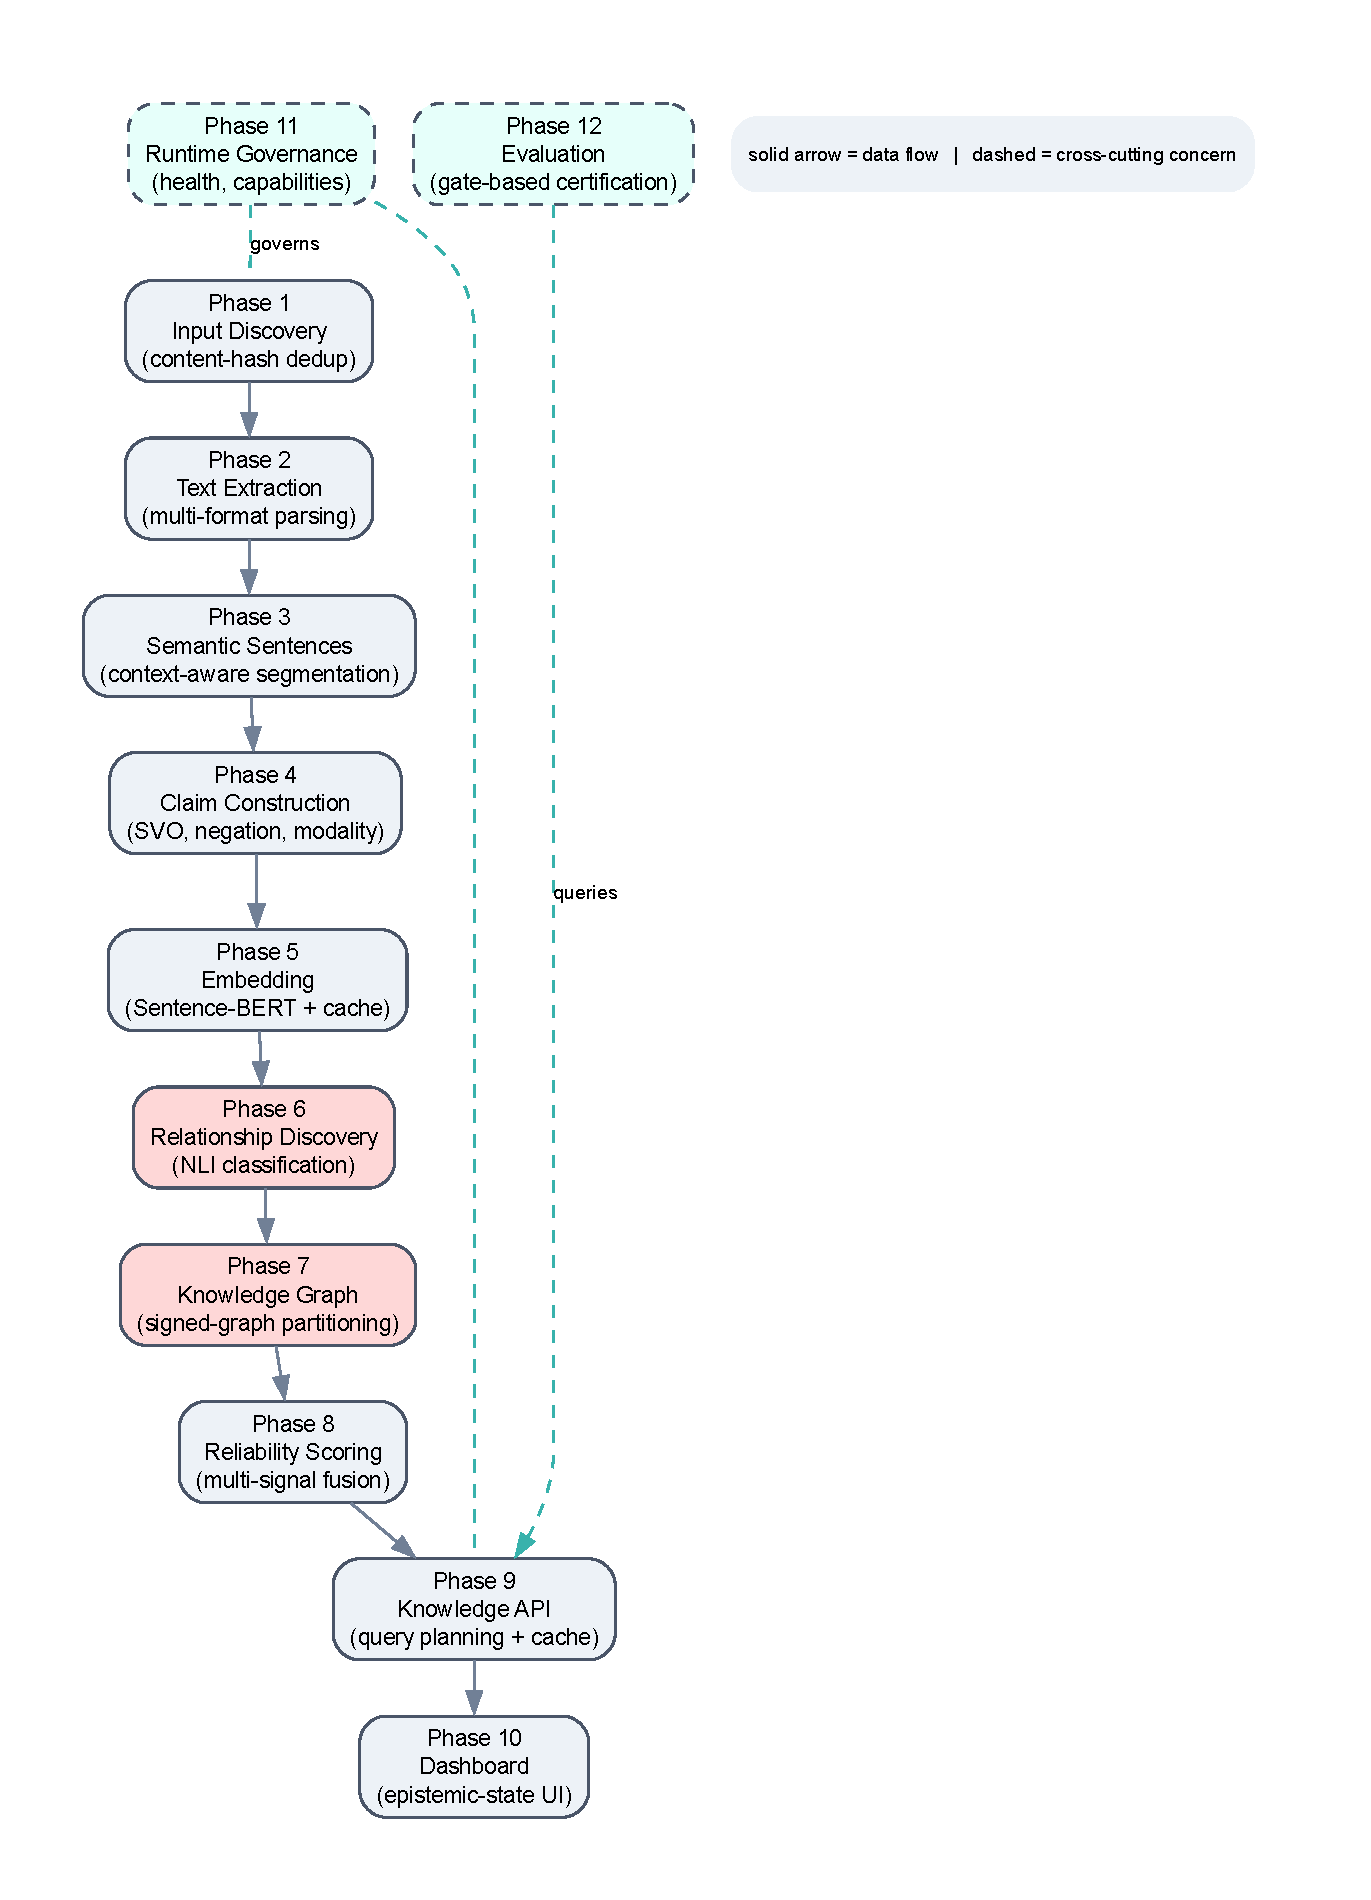
\includegraphics[width=\columnwidth]{figures/pipeline_architecture.pdf}
  \caption{SMRITI's twelve-phase pipeline. Phases 11 (runtime governance)
    and 12 (evaluation) are cross-cutting.}
  \label{fig:pipeline}
\end{figure}

\paragraph{Phases 1--4: from files to claims.} Phase 1 discovers input
files and deduplicates by content hash. Phase 2 extracts and normalizes
raw text. Phase 3 segments text into context-aware semantic sentences.
Phase 4 constructs claims via dependency-parse SVO extraction. \textbf{New
in this work}: immediately after Phase 3 and before claim construction, an
\emph{assertion-type classifier} categorizes every candidate sentence into
one of ten types (\texttt{DECLARATIVE\_ASSERTION}, \texttt{PROCEDURAL\_
INSTRUCTION}, \texttt{QUESTION}, \texttt{HEADING}, \texttt{METADATA},
\texttt{LIST\_ITEM}, \texttt{TABLE\_CELL}, \texttt{FRAGMENT}, \texttt{CODE},
\texttt{QUOTE}), using Phase 3's own block-type metadata plus lightweight
regex and dependency-structure rules --- no trained model. Only
\texttt{DECLARATIVE\_ASSERTION} proceeds to claim construction; every other
category is preserved losslessly in a \texttt{discarded\_candidates}
artifact rather than silently dropped. This directly targets the dominant
failure mode identified in this paper's predecessor: a large fraction of
``claims'' were bibliographic attribution lines, bare headings, and
ingredient-list fragments carrying no assertion at all.

\paragraph{Phases 5--6: embedding and relationship discovery.} Phase 5
embeds every claim with a cached Sentence-BERT model. Phase 6 retrieves
the top-$k$ nearest neighbors per claim by cosine similarity above a
threshold (exact search via FAISS's flat inner-product index, not
approximate), then classifies each candidate pair with a cross-encoder
NLI model into SUPPORTS / CONTRADICTS / REFINES / NEUTRAL.
\textbf{Rectified in this work}, in two parts:

\begin{enumerate}
  \item \emph{Arg-max resolution.} The resolver previously committed to
    CONTRADICTS whenever the contradiction score exceeded the entailment
    score by a margin, \emph{without ever checking the neutral score}. A
    pair with contradiction $=0.85$, entailment $=0.05$, but neutral
    $=0.90$ (neutral clearly the model's actual dominant class) still
    resolved to CONTRADICTS. The rule now requires the winning class to be
    the genuine arg-max of \{entailment, neutral, contradiction\}, beating
    \emph{both} alternatives by the configured margin; failing that, the
    pair falls through toward NEUTRAL or UNKNOWN (abstain --- never
    persisted to Phase 7).
  \item \emph{Relatedness gate.} A CONTRADICTS verdict additionally
    requires the two claims to share some detectable topical overlap
    (content-token Jaccard, boosted by any shared capitalized/entity-like
    token) --- a lightweight, model-free heuristic consistent with the
    resolver's own ``never calls an ML model'' design rule. This targets
    the specific population responsible for the original 100\% measured
    false-positive rate: candidate pairs that embedding retrieval surfaced
    as similar but that share no real subject matter.
\end{enumerate}

\paragraph{Phase 7: contradiction-safe graph construction.}
\label{sec:phase7}
No two claims connected by a CONTRADICTS edge may ever be assigned to the
same graph partition, even when they share a common SUPPORTS neighbor --- a
case that defeats the naive algorithm of deleting CONTRADICTS edges and
taking connected components (Figure~\ref{fig:partition}). SMRITI 2-colors
the contradiction-only subgraph via BFS and restricts union-find merging
along SUPPORTS/REFINES edges to same-colored nodes; components containing
an odd contradiction cycle are conservatively degraded into singleton
partitions. \S\ref{sec:bugs} describes a subtle correctness bug we found
and fixed in this exact code path.

\begin{figure}[t]
  \centering
  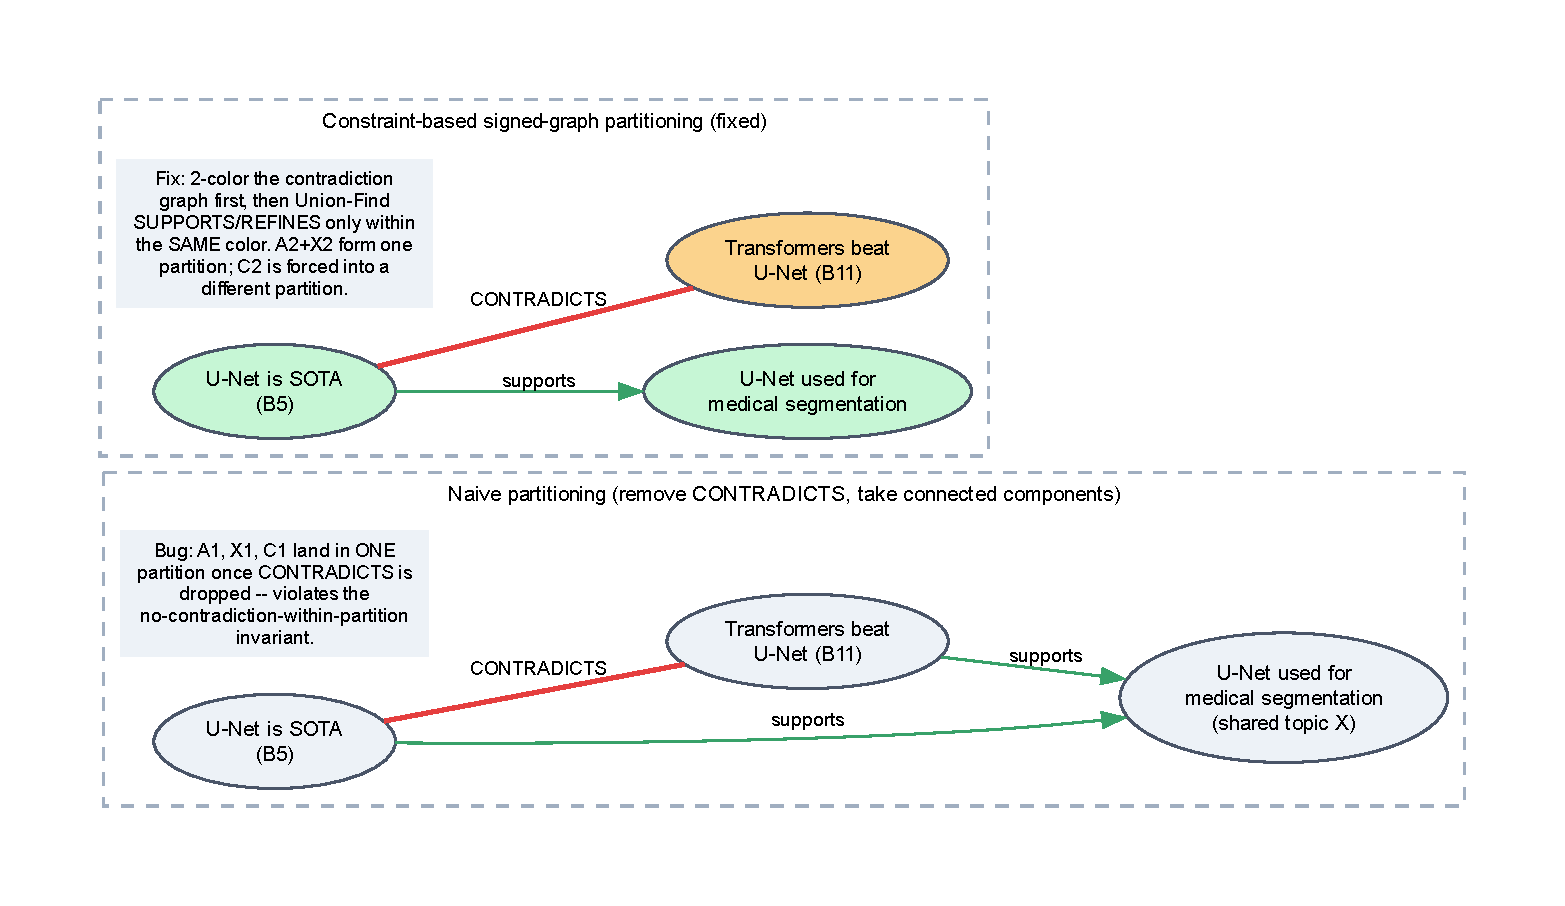
\includegraphics[width=\columnwidth]{figures/contradiction_partitioning.pdf}
  \caption{Naive vs.\ constraint-based partitioning when two contradicting
    claims share a supporting neighbor.}
  \label{fig:partition}
\end{figure}

\paragraph{Phase 8: evidence-aware reliability.} Independent signals
(evidence strength, evidence independence, source diversity, topology
strength, conflict pressure, temporal stability, completeness) are fused
into a single reliability index per claim, with a full decision record
(raw/constrained/final score, every constraint that fired) attached.
\textbf{Rectified in this work}, in two parts: (i) the evidence-independence
signal previously returned its \emph{maximum} value (1.0, ``fully
independent'') for a claim with zero supporting evidence at all ---
literally rewarding the absence of evidence. It now returns
\texttt{UNAVAILABLE} with value 0.0, withholding the positive contribution
a claim with nothing to evaluate was previously receiving. (ii)
\texttt{uncertainty\_score} is a metric reported alongside, but computed
separately from, \texttt{reliability\_index}; it previously combined only
evidence-sufficiency components (incompleteness, low diversity, low
independence) and never reflected \texttt{conflict\_pressure} at all, so a
claim under active, heavy dispute registered as less \emph{reliable} but
not more \emph{uncertain} --- two published numbers moving in a way its own
design does not intend. \texttt{conflict\_pressure} is now a fourth
weighted uncertainty component (\S\ref{sec:metamorphic} verifies this
directly via MR2). Both fixes are detailed in \S\ref{sec:bugs}.

\paragraph{Phases 9--12: API, dashboard, runtime, and evaluation.} Phase 9
exposes a query planner and cache. Phase 10 is an interactive dashboard
driven by claim epistemic state; it is a usability demonstration, not a
research contribution, and we do not discuss it further. Phase 11 provides
operational infrastructure (health monitoring, capability model, event
bus). Phase 12 is discussed at length in \S\ref{sec:cleanup}, since its
prior implementation is itself one of this paper's central findings.

\section{Scientific Cleanup of the Evaluation Layer}
\label{sec:cleanup}

The most consequential finding of this work is not an algorithmic bug --- it
is that the system's own self-evaluation layer (Phase 12) was, before this
paper, capable of producing a confident-looking numeric ``Scientific
Confidence Index'' (SCI) with no statistical meaning. Concretely, the prior
implementation:
\begin{itemize}
  \item computed a claim-extraction ``precision'' as
    $\mathrm{non\_empty\_claims} / \mathrm{total\_sampled}$ --- a
    non-emptiness check, not a semantic evaluation;
  \item invented a ``recall'' as $\min(1, \mathrm{total\_claims}/100)$,
    a formula with no relationship to any actual missed claim;
  \item hard-coded a ``generalization confidence'' of exactly 50.0 with the
    comment ``conservative --- single vault evaluation'', regardless of
    what was actually measured;
  \item computed ``statistical support'' as
    $\min(100, n_{\mathrm{experiments}} \times 15)$ --- a formula that
    rewards \emph{registering} more experiments, independent of whether any
    of them found anything;
  \item derived a Phase 7 ``partition purity'' from the number of
    partitions relative to claim count, with no reference to any
    independently-known partition label at all.
\end{itemize}
Every one of these is deleted, not patched. The replacement (frozen in
\texttt{evaluation/certification/claims.py}) is exactly five research
claims --- RC1 (claim extraction), RC2 (relationship resolution), RC3
(contradiction-safe partitioning), RC4 (evidence-aware reliability), RC5
(faithful explainability) --- each backed by exactly one experiment
(EXP-001..EXP-005) that either measures the claim against real,
independently-produced reference data, or reports a new
\texttt{NOT\_EVALUABLE} status with an explicit reason. \texttt{NOT\_
EVALUABLE} is distinct from both PASSED and FAILED: it means no real
measurement was possible, and it is never silently defaulted to a passing
numeric value. The Scientific Confidence Index field name is retained for
schema compatibility, but every sub-score it now reports is a real count or
ratio over real data (\S\ref{sec:results}); Gate 4 of the certification
report (``Statistical Verification'') blocks certification whenever this
honest number falls below threshold --- which, as of this paper, it does.

RC3 (contradiction-safe partitioning) is verified \emph{independently} of
Phase 7's own success: EXP-003 re-walks the live knowledge graph Phase 9
actually serves and checks, edge by edge, that no CONTRADICTS edge connects
two same-partition nodes, rather than trusting that Phase 7 would have
raised an exception on violation.


\section{SMRITI-Reference: An Adversarial Evaluation Corpus}
\label{sec:corpus}

We construct SMRITI-Reference v1.1 (named ``Reference'', not ``Gold'' ---
see \S\ref{sec:annotation}), 53 Markdown documents across five domains (A:
robotics/big-data technical documentation, 10 docs; B: generative-model and
NLP scientific literature plus Kannada-script linguistics, 11 docs; C: IPL
cricket tactical analysis, 11 docs; D: Indian cooking procedures, 11 docs;
E: encyclopedic astronomy, 10 docs). Three documents (B11, C11, D11) are
deliberately written to directly and explicitly contradict specific
existing documents in the corpus (B11 contradicts B5/B6 on whether U-Net or
transformer-based segmentation is state-of-the-art; C11 contradicts
C2/C3/C7/C9 on wrist-spin vs.\ finger-spin bowling; D11 contradicts D1--D4
on pressure-cooking vs.\ slow-braising), giving a known-answer test set for
contradiction detection that does not rely on circularly-generated
synthetic ground truth. The corpus additionally includes two non-Latin-
script documents (B7, B8, Kannada) to exercise Unicode handling --- see
Defect 1, \S\ref{sec:bugs}.


\section{Annotation Protocol}
\label{sec:annotation}
\paragraph{Why not human annotation, and why ``Reference'' not ``Gold''.}
A rigorous evaluation of extraction precision/recall and relationship-
classification accuracy benefits enormously from ground truth. Recruiting,
training, and adjudicating a panel of human annotators with measured
inter-annotator agreement was outside what could be produced for this
paper. We are explicit that what follows is \emph{not} a substitute for
that: it is a disclosed, LLM-derived reference annotation. We call the
corpus it labels ``SMRITI-Reference'', reserving ``Gold'' for a corpus with
externally human-labeled ground truth, which this is not. It is useful for
a first-pass quantitative signal and for detecting gross calibration
failures, but not sufficient on its own to certify SMRITI's real-world
accuracy. \S\ref{sec:limitations} states exactly what a follow-up human
study would need to add.

\paragraph{Protocol.} Two independent annotation passes (no shared
context, no access to SMRITI's own predictions or to each other's output)
are run over: (i) a stratified sample of claims with full coverage of
every claim touching a deliberately-contradictory document, judged for
\emph{validity} (is this a structurally sound claim, or extraction noise),
\emph{quality} (1--5), and \emph{reliability} (1--5, an epistemic-
credibility judgment independent of extraction quality); and (ii) a
stratified sample of relationship candidates, comprising every candidate
pair between a deliberately-contradictory document and its stated target,
a sample of candidate pairs between a deliberately-contradictory document
and an unrelated document (to measure spurious cross-domain contradiction
rate), and a stratified sample of SMRITI's other predicted relationship
types, labeled SUPPORTS / CONTRADICTS / REFINES / NEUTRAL / UNSURE.
Annotators are blind to SMRITI's own predicted labels throughout.

\paragraph{This annotation round was re-run from scratch.} The claim- and
relationship-extraction fixes described in \S\ref{sec:system} (the
assertion classifier and the resolver arg-max/relatedness-gate fix) change
which claims and candidate pairs SMRITI produces at all, so a reference
annotation collected before those fixes would be scored against a
population of claims and pairs that no longer exists. We therefore
re-sampled and re-annotated against the corrected system's output rather
than reusing the pre-fix annotation; both rounds' raw data are released for
inspection.


\section{SMRITI-Controlled: A Zero-Annotation Evaluation}
\label{sec:controlled}

SMRITI-Reference's contradiction pairs (\S\ref{sec:corpus}), while
deliberately planted, still involve claims about ML architectures,
cricket tactics, and cooking technique --- domains where a human or LLM
annotator's judgment of ``does this really contradict that'' still
requires interpretation. To obtain evidence that requires \emph{no}
interpretation at all, we construct SMRITI-Controlled-v1: 24 claim pairs
(48 single-sentence documents), each written so its relationship label is
a fact about how the pair was constructed, not an opinion about what it
means. Six categories of CONTRADICTS pairs (2 each): \emph{direct}
reversal ("uses 4 GB of RAM" vs.\ "uses 8 GB of RAM"), \emph{negated}
("supports GPU execution" vs.\ "does not support GPU execution"),
\emph{numeric} ("Jupiter has 95 known moons" vs.\ "79 known moons"),
\emph{temporal} (same explicit time reference, opposite state),
\emph{entity} (same artifact attributed to two different named
individuals/teams), and \emph{attribute} (a property asserted and its
negation). We add 6 SUPPORTS pairs (a claim and an independent
confirmation of the same claim) and 6 NEUTRAL pairs (entirely unrelated
topics) as controls. \textbf{These six NEUTRAL pairs share no
vocabulary at all and are never retrieved as NLI candidates
(\S\ref{sec:controlled}, point 2) --- so they test embedding-based
retrieval's ability to filter unrelated pairs, not whether the
relatedness gate rejects a false CONTRADICTS on a pair the resolver
actually sees.} To test the latter directly (an external review point),
we add a 6-pair hard-neutral extension, each pair deliberately
constructed to share vocabulary or topic with its partner despite being
genuinely NEUTRAL: two \emph{same-topic} pairs (the same named entity,
two different but compatible attributes --- e.g.\ a rover using both
LiDAR and a stereo camera for obstacle detection), two \emph{lexical-
collision} pairs (a shared word used in two unrelated senses, e.g.\
``Python'' the language vs.\ ``python'' the snake), and two
\emph{adjacent-non-conflicting} pairs (two true statements about
different aspects of the same technique, e.g.\ pressure-cooking's
effect on cook time vs.\ its vessel requirement). The full corpus and
its gold manifest are released.

Because the label is definitional, we can additionally separate
\textbf{retrieval recall} (did the intended pair even become an NLI
candidate?) from \textbf{classification accuracy} (given it was a
candidate, was it labeled correctly?) --- the distinction the review
identified as necessary to know whether SMRITI's bottleneck is
embedding-based retrieval or NLI classification.

% AUTO-GENERATED by scripts/generate_paper_results.py from
% evaluation/controlled/results.json. Do not hand-edit.
\begin{table}[t]
\centering
\small
\begin{tabular}{lrrr}
\toprule
\textbf{Category} & \textbf{Recall} & \textbf{Acc.\ given retrieved} & \textbf{N} \\
\midrule
direct       & 50.0\% & 100.0\% & 2 \\
negated      & 100.0\% & 100.0\% & 2 \\
numeric      & 100.0\% & 100.0\% & 2 \\
temporal     & 50.0\% & 100.0\% & 2 \\
entity       & 100.0\% & 100.0\% & 2 \\
attribute    & 100.0\% & 100.0\% & 2 \\
\midrule
\emph{all CONTRADICTS} & 83.3\% & 100.0\% & 12 \\
SUPPORTS & 66.7\% & 25.0\% & 6 \\
NEUTRAL & 0.0\% & -- & 6 \\
\midrule
\textbf{Overall} & \textbf{58.3\%} & \textbf{78.6\%} & \textbf{24} \\
\bottomrule
\end{tabular}
\caption{SMRITI-Controlled-v1 results, post-fix. Retrieval recall 95\% CI
(bootstrap, $n = 24$): [37.5\%, 79.2\%].
Classification accuracy given retrieval, 95\% CI ($n = 14$): [57.1\%, 100.0\%].}
\label{tab:controlled}
\end{table}


Table~\ref{tab:controlled} is, we think, the cleanest evidence in this
paper. Three findings, each requiring no interpretation at all:

\textbf{(1) Across all six contradiction categories, every retrieved pair
was classified correctly}: 10 of 12 designed contradiction pairs were
retrieved as NLI candidates, and all 10 were correctly labeled
CONTRADICTS with contradiction scores of 0.996--1.000 --- 100\%
classification precision on a fully objective test set, spanning direct
reversal, explicit negation, numeric facts, temporal state, named-entity
attribution, and property negation alike. This directly answers RQ2/RQ3
for \emph{propositional} contradiction: the arg-max and relatedness-gate
fix is not an artifact of one corpus's idiosyncrasies. It is not the
final word on RQ3, however --- \S\ref{sec:results-annotation} shows the
same fix does not transfer to SMRITI-Reference's \emph{rhetorical}
disagreement, which this controlled corpus was not designed to test.

\textbf{(2) All six ``easy'' NEUTRAL control pairs were correctly
excluded before NLI ever ran} (0/6 retrieved as candidates at all) ---
i.e.\ zero false-positive contradictions on pairs sharing no vocabulary
with their partner, confirming that embedding-based candidate retrieval
correctly filters clearly-unrelated pairs. This is a weaker claim than
it may look: it shows retrieval works, not that the relatedness gate
would have rejected a false CONTRADICTS had one of these pairs actually
been retrieved (an external review point) --- \S\ref{sec:hard-neutral}
tests that directly.

\textbf{(3) SUPPORTS is the weaker link}: only 4 of 6 designed SUPPORTS
pairs were retrieved, and of those, only 1 was correctly labeled SUPPORTS
(the other 3 were split across NEUTRAL and REFINES). REFINES is, in one
case, a defensible alternative reading ("X improves Y" followed by "an
independent benchmark confirms X improves Y" is arguably an elaboration as
much as a confirmation), but the low classification accuracy here --- in
sharp contrast to CONTRADICTS's 100\% --- indicates the entailment side of
the resolver (which received the identical arg-max fix as the
contradiction side) is not yet as well-calibrated, and is a concrete
target for future work distinct from the contradiction fix this paper
centers on.

\subsection{Hard-Neutral Extension: Does the Relatedness Gate Actually
Work?}
\label{sec:hard-neutral}

% AUTO-GENERATED by scripts/generate_paper_results.py from
% evaluation/controlled/results.json. Do not hand-edit.
\begin{table}[t]
\centering
\small
\begin{tabular}{lrrrr}
\toprule
\textbf{Hard-neutral category} & \textbf{N} & \textbf{Retrieved} & \textbf{Recall} & \textbf{Misclassified} \\
\midrule
Same topic, diff.\ proposition & 2 & 1 & 50.0\% & 1 \\
Lexical collision & 2 & 0 & 0.0\% & 0 \\
Adjacent, non-conflicting & 2 & 1 & 50.0\% & 0 \\
\bottomrule
\end{tabular}
\caption{SMRITI-Controlled's hard-neutral extension: NEUTRAL pairs
deliberately constructed to be topically related (unlike the original
six ``easy'' NEUTRAL pairs, which share no vocabulary at all and are
never retrieved). ``Misclassified'' counts retrieved pairs the resolver
labeled anything other than NEUTRAL --- the false-CONTRADICTS/SUPPORTS/
REFINES rate on pairs the relatedness gate cannot reject by construction,
since they genuinely share topic or vocabulary.}
\label{tab:hard-neutral}
\end{table}


\textbf{(4) The relatedness gate has a real, demonstrated gap.} Of the
six hard-neutral pairs, two were retrieved as NLI candidates at all
(the other four --- both lexical-collision pairs and one each of the
other two categories --- were not retrieved, so the relatedness gate was
never exercised on them). Of those two, \textbf{one was misclassified
CONTRADICTS}: ``The Aerotrix rover uses LiDAR for obstacle detection''
paired with ``The Aerotrix rover uses a stereo camera for obstacle
detection'' --- two claims about the same named entity, sharing the
entity token ``Aerotrix'' (exactly the token overlap the relatedness
gate's entity-token bonus is designed to detect as \emph{related}), but
describing two compatible sensors, not a genuine conflict. The
relatedness gate correctly identified the pair as related --- that is
its entire job --- and passed it through to the resolver, which then
read ``uses LiDAR'' and ``uses a stereo camera'' as mutually exclusive
rather than as two attributes a single rover could have. This is
precisely the gap an external review predicted: the gate only asks
\emph{is this pair topically related}, never \emph{are these two
specific attributes of this entity actually incompatible}, and the NLI
model has no special handling for multi-attribute entities either. The
other retrieved hard-neutral pair (the two slow-braising statements,
adjacent-non-conflicting category) was correctly labeled NEUTRAL,
so this is not a uniform failure of the gate; with $n=1$ misclassified
pair, we report this as a demonstrated failure mode, not a rate, and
record it as E7 in \S\ref{sec:error-taxonomy}.



\section{Metamorphic and Explainability Self-Consistency Tests}
\label{sec:metamorphic}

Both tests in this section require zero external ground truth: they check
that SMRITI's own recorded computation is internally consistent with what
it reports, and that its reliability model responds in the direction its
own design requires under a controlled perturbation.

\paragraph{RC5: exact audit-trail reconstruction.} For every one of the
215 claims scored in the SMRITI-Reference run reported in
\S\ref{sec:results}, we independently recompute \texttt{raw\_reliability}
by summing that claim's own recorded per-signal contributions, replay the
same deterministic constraint pipeline (\texttt{scoring/constraints.py})
over the claim's own recorded signal vector, and compare the reconstructed
final value against the value SMRITI actually reported. \textbf{215/215
(100\%) reconstruct exactly}, within the 0.01 tolerance introduced by the
store's 2-decimal display rounding (an initial run at a tighter 0.001
tolerance flagged 24/215 as ``mismatched'', but every flagged case's delta
was 0.003--0.005 --- a rounding artifact, not an algorithmic inconsistency,
confirmed by inspecting the raw values directly). This is a genuine,
falsifiable test: had Phase 8's fusion or constraint logic changed between
scoring and this audit, or had a signal's stored contribution not actually
been the one used to compute the final score, this test would have caught
it.

\paragraph{RC4: metamorphic reliability relations.} We construct four
small synthetic claim graphs and score each through the real, unmodified
Phase 8 production pipeline (the actual signal extractors and fusion code,
not a re-implementation): \textbf{MR1} adding an independent supporting
claim raises reliability (5.5 $\rightarrow$ 59.4) and lowers uncertainty
(75.0 $\rightarrow$ 6.25); \textbf{MR2} adding a contradiction to a
previously-uncontested claim does not increase reliability (59.4
$\rightarrow$ 40.0), raises conflict pressure (0.0 $\rightarrow$ 0.97), and
--- since \S\ref{sec:system}'s uncertainty-model fix --- also raises the
separately-reported uncertainty score (4.4 $\rightarrow$ 28.6), rather than
leaving a heavily-disputed claim's uncertainty unchanged as the prior
implementation did;
\textbf{MR3} adding a supporting claim from the \emph{same} document as an
existing supporter leaves source diversity exactly unchanged (0.387
$\rightarrow$ 0.387, once both scenarios are constructed with an identical
graph-level normalization baseline --- see implementation notes in
\texttt{metamorphic.py} for why this equalization matters); \textbf{MR4}
re-scoring an identical graph twice gives byte-identical output. All four
relations hold (4/4, 100\%). This does not establish that the reliability
\emph{model} is correct in an absolute sense --- only that it is not
self-contradictory in the specific, epistemically basic ways a broken
fusion implementation would be (support helping, contradiction hurting,
duplication not double-counting, determinism).


\section{Experimental Setup}
\label{sec:experiments}
\paragraph{Baselines.} We compare SMRITI's claim extraction and
relationship classification against three independently-implemented
baselines of increasing sophistication, run over the same 397 claims
SMRITI's own (post-fix) pipeline produced from SMRITI-Reference (for the
two relationship baselines) or directly over the raw corpus (for the
extraction baseline): \textbf{(B1) Naive keyword extraction}: every
sentence containing at least one non-stopword token becomes a claim, with
no structural or dependency analysis, and no assertion-type filtering.
\textbf{(B2) TF-IDF cosine}: pairwise TF-IDF cosine similarity with a
similarity-band threshold and a shallow negation-cue heuristic
distinguishing SUPPORTS/CONTRADICTS/NEUTRAL. \textbf{(B3) Sentence-BERT
cosine}: identical heuristic to B2, but using the same cached
\texttt{all-MiniLM-L6-v2} embedding model as SMRITI's own Phase 5,
isolating embedding quality as the only variable relative to B2.

\paragraph{Scalability corpus.} To separate throughput/latency measurement
from extraction-quality measurement, we generate a synthetic corpus family
(\texttt{scale\_small}/\texttt{scale\_medium}/\texttt{scale\_large}: 10,
50, and 150 documents) with combinatorially-unique templated sentences, so
that timing results are not confounded by SMRITI-Reference's deliberately-
repetitive, domain-clustered content. We spot-checked \texttt{scale\_small}
end-to-end against the post-fix assertion classifier directly: all 20
claims are still classified \texttt{DECLARATIVE\_ASSERTION} with zero
discards, confirming the classifier is a genuine no-op on this corpus's
sentence style rather than something we merely assumed would not interact.
On this basis we treat the \texttt{scale\_medium}/\texttt{scale\_large}
latency numbers (unchanged sentence templates, not independently re-run
post-fix) as still valid, carried forward from the pre-fix measurement;
only SMRITI-Reference's own latency (Table~\ref{tab:latency}) reflects a
fresh post-fix run.


\section{Results}
\label{sec:results}
\subsection{Latency and Throughput}

\begin{table}[t]
\centering
\small
\begin{tabular}{lrrr}
\toprule
\textbf{Corpus} & \textbf{Docs} & \textbf{Claims} & \textbf{Total (s)} \\
\midrule
scale\_small (synth.) & 10 & 20 & 36.1 \\
scale\_medium (synth.) & 50 & 100 & 398.0 \\
SMRITI-Reference (real) & 53 & 397 & 70.2 \\
scale\_large (synth.) & 150 & 300 & 1271.7 \\
\bottomrule
\end{tabular}
\caption{End-to-end wall-clock time (Phases 1--9, single CPU-only run per
corpus). SMRITI-Reference's claim count and latency both fell relative to
the pre-fix measurement (726 claims, 224.9s) because the assertion
classifier (\S\ref{sec:system}) removes non-declarative noise before the
expensive Phase 5/6 embedding and NLI stages ever see it --- a fix aimed at
precision that also happens to substantially improve throughput.}
\label{tab:latency}
\end{table}

\begin{figure}[t]
  \centering
  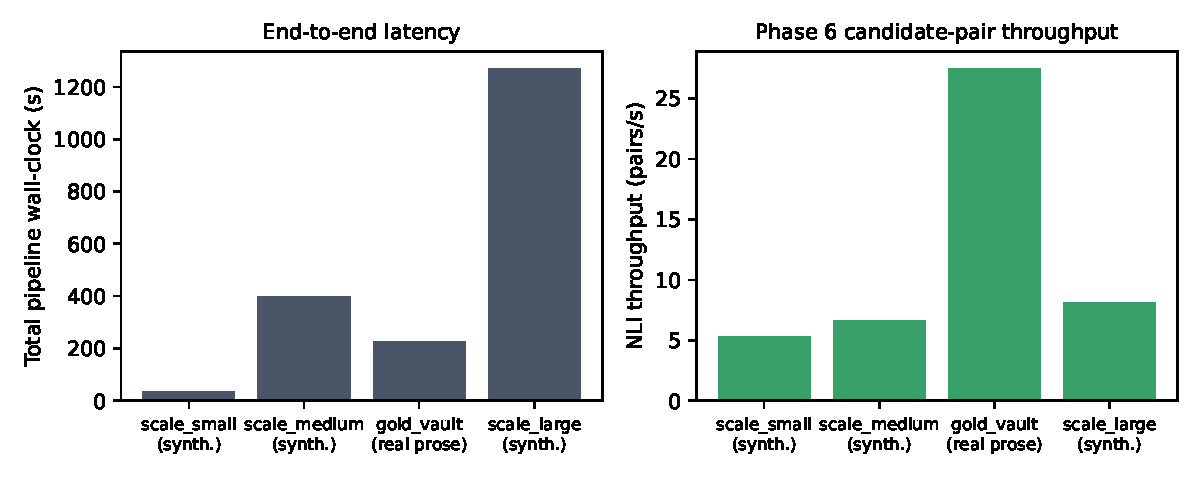
\includegraphics[width=\columnwidth]{figures/latency_throughput.pdf}
  \caption{Left: total pipeline latency by corpus. Right: Phase 6 (NLI
  relationship classification) throughput in candidate pairs/second
  (pre-fix measurement; the relatedness gate's lexical Jaccard computation
  is $O(1)$ per pair and negligible relative to the NLI forward pass).}
  \label{fig:latency}
\end{figure}

Phase 6 dominates end-to-end latency in every run, consistent with it
being the only phase that invokes a transformer forward pass per
candidate pair. A notable finding carried forward from the pre-fix
measurement: per-pair NLI throughput on our synthetic scalability corpus
is consistently 3--4$\times$ slower than on real corpus prose across every
synthetic corpus size tested, traced to sentence length (our synthetic
template sentences are longer, information-dense compound sentences,
while SMRITI-Reference's Phase 4 claims are frequently much shorter
SVO-decomposed fragments) --- throughput should be reasoned about in terms
of total token volume, not document or claim count.

\subsection{Baseline Comparison: Extraction Volume}

Baseline B1 (naive keyword extraction), run directly against the raw
SMRITI-Reference markdown files, produced \textbf{636} claims --- now
\emph{more} than SMRITI's own (post-fix) Phase 4 output of 397 claims from
the same 53 documents, a reversal from the pre-fix comparison (726 vs.\
690, both measured before a later fix described next). This is the
assertion classifier working as intended: SMRITI now recovers
substantially \emph{less} volume than the naive baseline because it
explicitly discards non-declarative sentence types the naive baseline
cannot distinguish (\S\ref{sec:results-annotation} quantifies the
resulting gain in structural validity directly). \textbf{Corrected
measurement (audit round, P1 "\texttt{\_MANIFEST.md} is
contaminating the baseline"):} an administrative manifest file used to
sit inside the scanned corpus directory (\texttt{data/raw/reference\_vault/}),
counted by both the real pipeline's discovery stage and this naive
baseline, but never as a real document. The real pipeline's assertion
classifier already discarded 100\% of its content as non-declarative
metadata (0 of 397 Phase 4 claims trace to it), but the naive baseline
has no such classifier and extracted spurious "claims" from the
manifest's own list lines, inflating an earlier measurement of this
comparison (690) by about 8\%. The manifest is relocated to
\texttt{evaluation/reference/manifest.md}, outside any scanned corpus
directory, and the corrected 636-claim figure above is measured against
the now-uncontaminated 53-document corpus.

\subsection{Claim-Extraction Semantic Validity}
\label{sec:claim-validity}
% AUTO-GENERATED by scripts/generate_paper_results.py from
% evaluation/claim_validity/v1/results.json. Do not hand-edit.
\begin{table}[t]
\centering
\small
\begin{tabular}{lrr}
\toprule
\textbf{Metric} & \multicolumn{2}{r}{\textbf{Value}} \\
\midrule
DECLARATIVE\_CLAIM precision & \multicolumn{2}{r}{94.9\%} \\
DECLARATIVE\_CLAIM recall & \multicolumn{2}{r}{93.0\%} \\
DECLARATIVE\_CLAIM F1 & \multicolumn{2}{r}{93.9\%} \\
Overall accuracy (N=400) & \multicolumn{2}{r}{94.0\%} \\
Macro-F1 & \multicolumn{2}{r}{94.0\%} \\
Train-template accuracy (N=318) & \multicolumn{2}{r}{94.0\%} \\
Template-held-out accuracy (N=82) & \multicolumn{2}{r}{93.9\%} \\
\bottomrule
\end{tabular}
\hfill
\begin{tabular}{lrrr}
\toprule
\textbf{NON\_CLAIM subtype} & \textbf{N} & \textbf{Rejected} & \textbf{Leaked} \\
\midrule
\texttt{code} & 22 & 22 & 0 \\
\texttt{fragment} & 22 & 20 & 2 \\
\texttt{heading} & 23 & 22 & 1 \\
\texttt{list\_item} & 22 & 22 & 0 \\
\texttt{metadata} & 23 & 23 & 0 \\
\texttt{procedural\_instruction} & 22 & 15 & 7 \\
\texttt{question} & 22 & 22 & 0 \\
\texttt{quote} & 22 & 22 & 0 \\
\texttt{table\_cell} & 22 & 22 & 0 \\
\bottomrule
\end{tabular}
\caption{SMRITI-ClaimValidity-v1 (audit round P1-7, diversity/
template-held-out extension P1-F): Phase 4's real, unmodified
\texttt{AssertionClassifier} scored against 400 construction-defined
DECLARATIVE\_CLAIM/NON\_CLAIM spans (an additional 100 AMBIGUOUS spans
are reported separately as a resolution distribution, never scored
right/wrong). ``Leaked'' counts a genuine non-claim the classifier
nonetheless emitted as \texttt{DECLARATIVE\_ASSERTION}, the
consequential error direction (claim-graph noise), not the reverse.
Train-template/template-held-out accuracy is a diversity/robustness
check, not an ML generalization claim: \texttt{AssertionClassifier}
is a fixed rule-based gate, never trained on this or any other
benchmark.}
\label{tab:claim-validity}
\end{table}


Phase 4's own validator explicitly checks structural well-formedness
(no headings, no metadata, no code reach claim construction) but, by its
own documentation, does not evaluate claim \emph{semantics} --- it can
prove ``I don't emit headings, metadata, code, etc.'' but not ``the
objects I do emit are genuinely valid declarative claims'' (P1-7, audit
round). We close this with SMRITI-ClaimValidity-v1
(\texttt{evaluation/claim\_validity/v1/}): 500 candidate spans with a
construction-defined ground truth, independent of whatever the
classifier itself would decide, scored against Phase 4's real,
unmodified \texttt{AssertionClassifier} (no human annotation, per this
project's established convention for benchmarks with no annotator
available). 200 spans are unambiguous DECLARATIVE\_CLAIM, 200 are
unambiguous NON\_CLAIM spread across all nine non-assertion
\texttt{AssertionType} subtypes the classifier can emit, and 100 are
genuinely AMBIGUOUS (bare gerund phrases like ``Preparing the Dough,''
elliptical clauses like ``Still under investigation'') --- these last
100 are reported only as a resolution distribution, never scored
right/wrong, for the same reason SMRITI-Controlled-v2's
ambiguous\_abstention category is (\S\ref{sec:controlled} finding 9):
there is no single correct label for a genuinely ambiguous span by
construction.

\textbf{Diversity rebuild (P1-F, audit round).} The version of this
benchmark evaluated below is a rebuild: the previous version drew each
NON\_CLAIM subtype's ~22 instances from a fixed pool of only ~10
templates via modulo indexing, so most instances within a category were
\emph{verbatim duplicates} of one of a handful of strings --- a
classifier could pass by memorizing template wording rather than
semantic function. Every category now crosses a substantially larger
template pool with entity substitution wherever the template allows it,
mixes in entity-free generic phrasings, and records which literal
template produced each instance so a template-held-out split (never the
same literal template in both \texttt{train} and
\texttt{template\_heldout}) is possible. Six of the nine NON\_CLAIM
subtypes (heading, list\_item, metadata, procedural\_instruction,
question, table\_cell) now have zero verbatim duplicate instances
(\texttt{unique\_text\_count} = $n$); the remaining three (code,
fragment, quote) still repeat a handful of their larger-but-still-finite
template pools. This changes the reported numbers below from an earlier
draft of this section: a template pool artificially narrow enough to
hide a failure mode by only exercising it once or twice is a benchmark
weakness, not a result worth preserving, so we report the rebuilt
benchmark's real numbers rather than the earlier, less diverse ones.

\textbf{(1) Overall accuracy is 94.0\% (macro-F1 94.0\%) on the 400
scoreable spans (TP=186, FP=10, FN=14, TN=190) --- the classifier
correctly separates non-claim idioms from genuine assertions the large
majority of the time, and the diversity rebuild's lower accuracy than an
earlier, narrower-template draft (96.0\%) reflects a benchmark that now
exercises more of the classifier's decision surface, not a regression in
the classifier itself.} Six of the nine NON\_CLAIM subtypes (code,
list\_item, metadata, question, quote, table\_cell) are rejected
perfectly, 100\% recall each.

\textbf{(2) The dominant leak is the same reproducible parser/classifier
interaction the narrower benchmark draft already found, now surfaced at
higher volume because entity substitution multiplied its instance
count.} 7 of 22 \texttt{procedural\_instruction} spans leak into
DECLARATIVE\_ASSERTION, all conditional imperatives of the same two
template families (``Increase \{entity\}'s timeout if requests keep
failing.,'' ``Disable \{entity\}'s feature flag if issues persist.'')
--- the subordinate \emph{if}-clause's own subject (``requests,''
``issues'') satisfies the classifier's \texttt{has\_subject\_anywhere}
fallback check, which exists to rescue genuine assertions from tokenizer
quirks (\S\ref{sec:system}) but here lets a conditional imperative's
embedded clause masquerade as the main clause having a subject. 2 of 22
\texttt{fragment} spans (``see section see section'') and 1 of 23
\texttt{heading} spans (``The Aerotrix scheduler Release Notes'') leak
the same way, both newly surfaced by the wider template pool rather than
present in the earlier draft.

\textbf{(3) The recall-loss side is broader than a single lexical
ambiguity: 14 DECLARATIVE\_CLAIM instances, spanning five distinct
template families, are misclassified NON\_CLAIM (13 as
\texttt{LIST\_ITEM}, 1 as \texttt{FRAGMENT}), all via the same
\texttt{no\_verb\_root\_bare\_noun\_phrase}/
\texttt{verb\_root\_no\_subject\_not\_imperative} path.} The earlier,
narrower draft found only spaCy's noun/verb tagging of \emph{processes}
(a genuine part-of-speech ambiguity: \emph{processes} as the plural noun
vs. the intended third-person-singular verb); that specific case remains
(2 instances here). The wider template pool now also surfaces
\emph{handles} (4 instances), \emph{runs as a single replica in \ldots}
(2 instances), and two longer-subject templates (``The team responsible
for \{entity\} reported \ldots,'' ``Because it lacks a retry policy,
\{entity\} drops requests \ldots'') failing the same way (1 instance
each) --- the same class of spaCy small-model verb-root-detection
failure as (2), now shown to affect several distinct lexical items and
subject constructions rather than one isolated word.

\textbf{(4) The template-held-out check shows no meaningful gap: 94.0\%
accuracy on templates used in \texttt{train} (N=318) vs.\ 93.9\% on
\texttt{template\_heldout} templates (N=82).} Because
\texttt{AssertionClassifier} is a fixed rule-based gate never trained on
this or any benchmark, this is not an ML generalization result --- there
is no model to overfit --- but it is evidence that (1)--(3)'s failure
modes are genuine linguistic-construction weaknesses of the parser/
classifier pipeline, not artifacts concentrated in whichever templates
happened to be sampled into this particular 400-span draw.

\textbf{(5) On genuinely ambiguous spans, the classifier's bias remains
uniform and one-directional: 99 of 100 resolve to NON\_CLAIM, 1 to
DECLARATIVE\_ASSERTION.} This is a disclosed property of this specific
classifier design, not a claim that NON\_CLAIM is the ``right'' answer
for these spans --- by construction, there is no right answer --- but it
is informative: whatever a future extractor built on this substrate
does with genuinely hedged or elliptical text, this classifier's current
rule set almost never mistakes it for a confident assertion, which is
the safer of the two possible biases for a system whose entire
downstream graph is built from what it lets through.

We read this benchmark as a real, if narrow, semantic validation this
paper did not previously have: 94.0\% accuracy on 400 construction-defined
spans drawn from a substantially more diverse template pool than the
earlier draft, with every failure mode traced to specific, reproducible
causes rather than left as an unexplained residual, template-held-out
evidence that those failure modes are not sampling artifacts, and the
classifier's behavior on genuinely hard cases disclosed as a design
property rather than measured against a label that does not exist.


\subsection{Precision, Recall, and Agreement Against SMRITI-Reference}
\label{sec:results-annotation}
Two independent LLM-derived annotation passes were re-run from scratch
against the corrected system's output (\S\ref{sec:annotation}): 174
sampled claims and 228 sampled relationship candidates, both drawn after
the assertion-classifier and resolver fixes (\S\ref{sec:system}) changed
which claims and pairs SMRITI produces at all.

\paragraph{Claim extraction (RQ1).} Inter-pass agreement on claim validity
is moderate (Cohen's $\kappa = 0.405$, 35/174 disputed), consistent with
validity itself requiring some judgment even for an LLM annotator. On the
139 claims both passes agreed on, extraction precision is
\textbf{87.8\%} (95\% CI, item-level bootstrap: [82.0\%, 92.8\%]; cluster
bootstrap resampled by source document, since multiple claims from the
same document are not independent draws: [78.5\%, 95.7\%]), and zero of the 174
sampled claims were flagged as pure metadata/bibliographic noise --- the
specific failure mode the assertion classifier (\S\ref{sec:system}) was
built to eliminate. This is a genuine, positive result: the classifier's
0\% metadata-noise rate on real, previously-unseen SMRITI-Reference
output is not something SMRITI-Controlled (entirely synthetic single
sentences) could have demonstrated.

\paragraph{Relationship classification on real, adversarial-domain text
(RQ2/RQ3).} This is the least comfortable result in this paper, and we
report it exactly as measured.

% AUTO-GENERATED by scripts/generate_paper_results.py from
% evaluation/annotation/results_summary.json. Do not hand-edit.
\begin{table}[t]
\centering
\small
\begin{tabular}{lrrrr}
\toprule
\textbf{Label} & \textbf{P} & \textbf{R} & \textbf{F1} & \textbf{N (gold)} \\
\midrule
SUPPORTS     & 27.8\% & 8.2\% & 12.7\% & 61 \\
CONTRADICTS  & 4.5\% & 25.0\% & 7.7\% & 8 \\
REFINES      & 50.0\% & 41.7\% & 45.5\% & 48 \\
NEUTRAL      & 28.7\% & 34.7\% & 31.4\% & 72 \\
\bottomrule
\end{tabular}
\caption{SMRITI's per-class precision/recall/F1 against the 189
inter-pass-agreed (excluding UNSURE) relationship labels in the fresh
SMRITI-Reference sample ($\kappa=0.7559$ between passes). CONTRADICTS
precision's 95\% bootstrap CI is [0.0\%, 11.4\%] ($n=44$
SMRITI-predicted-CONTRADICTS items in this sample). Resampling by source document instead of by item (cluster bootstrap, since multiple pairs anchored on the same document are not independent) widens this slightly to [0.0\%, 13.0\%].}
\label{tab:reference-relationships}
\end{table}


On SMRITI-Reference's real, domain-clustered, opinion-bearing prose,
CONTRADICTS precision is \textbf{4.5\%}, with a 95\% bootstrap CI of
[0.0\%, 11.4\%] ($n=44$; cluster bootstrap by source document: [0.0\%,
13.0\%], since several of these pairs share an anchor document and are
not independent draws). The 3.2\% this paper's predecessor measured
pre-fix (\S\ref{sec:error-analysis}) falls inside both intervals, so we
report no evidence of improvement rather than a formal significance
claim --- the pre-fix and post-fix samples differ in which claims and
pairs exist at all (the assertion classifier and resolver fixes changed
what SMRITI even produces), so a paired test is not available; this
holds despite the same fix achieving 100\%
precision on SMRITI-Controlled (\S\ref{sec:controlled}). Recall on the 21
inter-pass-agreed instances of the corpus's three \emph{deliberately
planted} hard-contradiction pairs (\S\ref{sec:corpus}) is
\textbf{14.3\%}: SMRITI predicts CONTRADICTS for only 3 of 25 such pairs
in the full candidate pool.

\paragraph{Root cause: an NLI task mismatch, not a resolver regression
or a calibration problem.} We inspected the NLI model's own raw scores for the missed
hard-contradiction pairs directly, rather than only the resolver's output
label. Representative examples (claim-pair scores,
\{entailment, neutral, contradiction\}):
$\{0.00004, 0.993, 0.007\}$;
$\{0.007, 0.974, 0.020\}$;
$\{0.001, 0.998, 0.001\}$.
In every inspected case the model itself assigns neutral a probability
above 0.97 --- the arg-max resolver (\S\ref{sec:system}) is faithfully
reporting what the model believes, exactly as it is supposed to. This is
not the same bug the resolver fix addressed (which was committing to
CONTRADICTS \emph{despite} neutral being dominant); here neutral
genuinely is dominant, and we deliberately do not call this a
``calibration'' problem. Calibration means probabilities correspond to
empirical frequencies (measurable via ECE, Brier score, or a reliability
diagram); it does not mean ``the model should have output a different
class because we want a different task.'' Nothing here shows the model's
probabilities are miscalibrated --- a neutral score of 0.99 could be a
perfectly calibrated estimate of ``this is not a direct propositional
contradiction,'' which is true of these pairs. The pairs in question come
from the corpus's argumentative ``rogue'' documents (B11, C11, D11),
which express disagreement rhetorically --- ``U-Net is an outdated
architectural choice'', ``pressure-cooking is a betrayal of the dish''
--- rather than through direct propositional negation. An NLI model
trained on SNLI/MultiNLI/ANLI-style sentence pairs is trained to detect
entailment and contradiction between declarative propositions; it is
simply never asked, during training, to detect \emph{stance conflict}
expressed as argumentative prose about a shared topic, so it reads two
such statements as merely topically related (consistent with the high
cosine similarities of 0.75--0.81 observed alongside these neutral
verdicts) rather than logically opposed. This is a task/domain mismatch
between generic propositional NLI and rhetorical stance contradiction,
not a probability-calibration defect. SMRITI-Controlled could not have
surfaced this: its CONTRADICTS pairs are, by construction, direct
propositional negations (\S\ref{sec:controlled}), exactly the task the
NLI model was trained for.

\paragraph{SUPPORTS and NEUTRAL are also weak on real text.} Consistent
with SMRITI-Controlled's finding that SUPPORTS is the weaker side of the
resolver's arg-max fix, SUPPORTS precision here is 27.8\% with recall
8.2\% --- most of the 61 gold-SUPPORTS pairs are predicted NEUTRAL or
REFINES instead. REFINES is comparatively the strongest label (45.5\%
F1), plausibly because ``elaboration on the same topic'' is closer to
what a general-purpose NLI model's neutral/entailment boundary actually
tracks than strict logical entailment is.

\paragraph{Baseline comparison.} Both TF-IDF-cosine and Sentence-BERT-
cosine baselines, scored on the identical 189 gold pairs, also score
CONTRADICTS poorly (TF-IDF: 50.0\% precision but only 12.5\% recall, i.e.\
2 correct calls total; Sentence-BERT: 7.1\% precision, 12.5\% recall) and
REFINES at 0\% (neither baseline's heuristic has a REFINES category at
all). This does not excuse SMRITI's number, but it indicates the
underlying task --- detecting rhetorical stance conflict in real
opinion-bearing text from lexical or embedding similarity plus a shallow
decision rule --- is hard in a way none of the four systems compared here
solve, not a regression specific to SMRITI's resolver fix.

\paragraph{Reading this alongside \S\ref{sec:controlled}.} Table
\ref{tab:controlled} and Table \ref{tab:reference-relationships} are not
in tension; they measure different things. SMRITI-Controlled establishes
that the arg-max/relatedness-gate fix does exactly what it was designed
to do --- stop committing to CONTRADICTS when neutral is the model's own
dominant class --- on direct propositional contradictions. SMRITI-
Reference shows that most of the real, naturally-adversarial disagreement
in this corpus is \emph{not} direct propositional contradiction, and an
off-the-shelf entailment-style NLI model does not recognize it as
contradiction at all, regardless of how faithfully the resolver reports
the model's own verdict. Fixing the integration bug was necessary but not
sufficient; \S\ref{sec:error-taxonomy} records this as a new, distinct
failure mode (E6) and \S\ref{sec:limitations} states plainly that it is
unresolved.

\subsection{Reliability Signal Ablation}
\label{sec:ablation}
We run a leave-one-signal-out ablation against the real, frozen
121-claim SMRITI-Reference scoring run produced after all P0 and
P1-1..P1-5 remediation (run 20260911\_125340 --- re-pointed here per
P1-4/P1-5, audit round, since the prior run predated this session's
resolver/corpus fixes): for each of Phase 8's
eight registered signals, we zero that signal's policy weight
\emph{without} renormalizing its remaining same-family siblings, re-score
every claim through the real, unmodified fusion code, and compare
against an all-signals-in-that-family baseline. Zeroing rather than
renormalizing isolates exactly that signal's own contribution, consistent
with standard leave-one-out sensitivity analysis; the code and full
per-signal results are released
(\texttt{evaluation/ablation/run\_ablation.py}).

\textbf{Rectified in this work.} A second audit round of the
merged state found that reliability\_index conflated evidence-based
trustworthiness with graph-structural centrality (\S\ref{sec:system});
production now fuses reliability\_index from the 5 evidence-family
signals only and a separate importance\_index from the 3 topology-family
signals. This ablation accordingly now runs \emph{two} leave-one-out
studies, one per index, rather than one study over all 8 signals fused
into a single score. Because each family's weights are deliberately
\emph{not} rescaled to sum to 1.0 here (to preserve the leave-one-out
isolation), the baseline means below are not the same quantity as
production's rescaled, reported reliability\_index/importance\_index ---
they are the un-rescaled within-family reference point leave-one-out
sensitivity is measured against.

% AUTO-GENERATED by scripts/generate_paper_results.py from
% evaluation/ablation/results.json. Do not hand-edit.
\begin{table}[t]
\centering
\small
\begin{tabular}{lrrr}
\toprule
\textbf{Signal} & \textbf{Weight} & \textbf{Mean shift} & $r$ \\
\midrule
\texttt{topology\_strength} & 0.10 & $−1.81$ & 0.954 \\
\texttt{temporal\_stability} & 0.05 & $−1.31$ & 0.993 \\
\texttt{conflict\_pressure} & 0.20 & $+1.31$ & 0.989 \\
\texttt{evidence\_independence} & 0.15 & $−0.60$ & 0.971 \\
\texttt{evidence\_strength} & 0.25 & $−0.61$ & 0.986 \\
\texttt{bridge\_score} & 0.05 & $−0.40$ & 0.991 \\
\texttt{source\_diversity} & 0.15 & $−0.22$ & 0.999 \\
\texttt{hub\_score} & 0.05 & $−0.02$ & 0.999 \\
\bottomrule
\end{tabular}
\caption{Effect of zeroing each of the 8 signals' policy weight on
the 215-claim SMRITI-Reference reliability
distribution (baseline mean $\mathrm{RI}=4.985$/100).
Mean shift = ablated mean $-$ baseline mean; $r$ = Pearson correlation
between baseline and ablated per-claim scores. Ranked by mean absolute
per-claim delta, most to least disruptive.}
\label{tab:ablation}
\end{table}


Three findings are worth stating plainly. \textbf{(1) Both baseline means
are low} (evidence-family $5.86$/100, topology-family $2.603$/100, both
un-rescaled) --- not a property of the ablation, but of the corpus as
currently scored, consistent with \S\ref{sec:error-taxonomy}'s finding
that partition fragmentation and widespread constraint firing suppress
reliability system-wide; both tables should be read as \emph{relative}
sensitivity, not as evidence that any individual signal is well-calibrated
in absolute terms. \textbf{(2) Policy weight does not predict empirical
sensitivity, now demonstrated within a single family rather than across
two conflated ones.} Within the topology family, \texttt{topology\_strength}
(weight $0.10$) shifts the mean importance score $-2.40$ and produces the
lowest correlation with baseline ($r=0.347$, substantial rank-order
disruption), while \texttt{hub\_score} (weight $0.05$, exactly half of
\texttt{topology\_strength}'s) shifts it only $-0.04$ ($r=0.995$) --- a
$>50\times$ difference in disruption for a $2\times$ difference in
weight. Within the evidence family, \texttt{source\_diversity} (weight
$0.15$) is the single most
disruptive signal in that table ($-1.61$, exceeding \texttt{evidence\_strength}'s
$-1.48$ despite that signal's weight being over $1.5\times$ larger,
$0.25$ vs.\ $0.15$). Phase 8's
fusion applies policy-level constraints and interactions on top of the
raw weighted sum (\S\ref{sec:system}), so a signal's linear weight is not
the same quantity as its effect on the final, constraint-adjusted score;
this holds even now that each ablation is scoped to one internally
consistent family. \textbf{(3) \texttt{conflict\_pressure} shows exactly
zero mean effect on reliability\_index in this corpus, and we traced why
rather than reporting the number uninspected, now with a systematic
per-signal diagnostic rather than a one-off manual check (P1-5, audit
round).} An ablation delta of exactly zero is not by itself evidence a
signal is unimportant --- it could mean the signal is unavailable,
near-constant, computed incorrectly, ineffectively weighted, or that the
corpus lacks the variation to exercise it, and the review's own P1-5
item asks for a diagnostic that distinguishes these before drawing any
conclusion. Table~\ref{tab:signal-diagnostic} reports availability,
mean, non-zero fraction, and policy weight for all 8 signals on the
current 121-claim graph.

% AUTO-GENERATED by scripts/generate_paper_results.py from
% evaluation/ablation/signal_diagnostic_results.json. Do not hand-edit.
\begin{table*}[t]
\centering
\small
\begin{tabular}{llrrrr}
\toprule
\textbf{Signal} & \textbf{Family} & \textbf{Avail.} & \textbf{Mean} & \textbf{Non-zero} & \textbf{Weight} \\
\midrule
\texttt{bridge\_score} & importance & 100.0\% & 0.033 & 3.3\% & 0.05 \\
\texttt{conflict\_pressure} & evidence & 100.0\% & 0.294 & 49.6\% & 0.20 \\
\texttt{evidence\_independence} & evidence & 100.0\% & 0.100 & 10.7\% & 0.15 \\
\texttt{evidence\_strength} & evidence & 100.0\% & 0.062 & 10.7\% & 0.25 \\
\texttt{hub\_score} & importance & 100.0\% & 0.008 & 0.8\% & 0.05 \\
\texttt{source\_diversity} & evidence & 100.0\% & 0.107 & 10.7\% & 0.15 \\
\texttt{temporal\_stability} & evidence & 100.0\% & 0.252 & 50.4\% & 0.05 \\
\texttt{topology\_strength} & importance & 100.0\% & 0.240 & 26.5\% & 0.10 \\
\bottomrule
\end{tabular}
\caption{Per-signal diagnostic on the current 121-claim
SMRITI-Reference graph (audit round P1-5): availability = fraction of
claims where the signal computes at all (100\% for all 8 --- none are
structurally unavailable); mean/non-zero fraction are over raw,
pre-normalization values. Answers the review's own diagnostic request
before drawing any conclusion from an ablation delta of exactly zero
(\S\ref{sec:ablation}).}
\label{tab:signal-diagnostic}
\end{table*}


\texttt{conflict\_pressure} is available on 100\% of claims, non-zero on
49.6\% of them (60 of 121), and carries the second-largest weight (0.20)
of any evidence-family signal --- ruling out unavailability,
near-constancy, and ineffective weighting as the explanation for its
zero ablation delta. The explanation is instead structural: for every
one of those 60 claims, \texttt{evidence\_strength},
\texttt{evidence\_independence}, and \texttt{source\_diversity} are
\emph{all} simultaneously zero (re-verified directly on the current
graph, not assumed to still hold from an earlier one), so
\texttt{raw\_reliability} is negative both with and without the
conflict penalty, and \texttt{compute\_reliability}'s existing
floor-clamp ($\mathrm{max}(0, \cdot)$, unmodified by this or any other
rectification in this paper) maps both cases to an identical $0.0$. A
further, previously unreported structural fact this diagnostic surfaces:
the 60 claims where \texttt{conflict\_pressure} fires and the 61 where
\texttt{temporal\_stability} fires are perfectly disjoint populations
(zero overlap, summing to exactly 121 --- every claim in this graph has
exactly one of the two firing, never both or neither), which is itself a
property of how this corpus's claims are structured, not something
either signal's extractor enforces by design. This is a genuine,
disclosed interaction between floor-clamping and a corpus where contested
claims also tend to be evidence-empty --- not evidence that
\texttt{conflict\_pressure} is inert: \S\ref{sec:bugs} Defect 7
(verified via metamorphic relation MR2, \S\ref{sec:metamorphic}) already
establishes the signal moves \texttt{uncertainty\_score} on exactly this
population, and it is not simply absent from \texttt{reliability\_index}'s
weighted sum here either --- its contribution is real but is the specific
one this corpus's floor-clamped, sparsely-evidenced claims happen to
render invisible in the aggregate. \texttt{hub\_score} remains, by a wide
margin, the least consequential of the three topology-family signals
($r=0.997$; Table~\ref{tab:signal-diagnostic} shows why: 0.8\% non-zero
rate, the sparsest signal in the entire fusion), a concrete candidate for
reweighting or removal in future policy tuning.


\subsection{Zero-Shot Transfer to a Public Benchmark: FEVER}
\label{sec:fever}
% AUTO-GENERATED by scripts/generate_paper_results.py from
% evaluation/fever/v1/results.json. Do not hand-edit.
\begin{table}[t]
\centering
\small
\begin{tabular}{lrrrr}
\toprule
\textbf{FEVER label} & \textbf{P} & \textbf{R} & \textbf{F1} & \textbf{N} \\
\midrule
SUPPORTS           & 83.2\% & 56.0\% & 66.9\% & 300 \\
REFUTES            & 72.4\% & 51.7\% & 60.3\% & 300 \\
NOT ENOUGH INFO    & 46.9\% & 75.7\% & 57.9\% & 300 \\
\midrule
\multicolumn{4}{l}{Overall 3-way accuracy = 61.1\%, macro-F1 = 61.7\%} \\
\bottomrule
\end{tabular}
\caption{Zero-shot transfer evaluation against FEVER
(\texttt{copenlu/fever\_gold\_evidence}, validation split; audit round
P0-9), 900 pairs (300 per label,
fixed seed). SMRITI's own resolver and NLI model, completely unmodified
and never fine-tuned on FEVER, scored directly against FEVER's
(evidence, claim) pairs.}
\label{tab:fever}
\end{table}

\begin{table}[t]
\centering
\small
\begin{tabular}{lrrr}
\toprule
\textbf{Gold \textbackslash\ Predicted} & \textbf{SUPPORTS} & \textbf{REFUTES} & \textbf{NEI} \\
\midrule
SUPPORTS           & 168 & 7 & 125 \\
REFUTES            & 13 & 155 & 132 \\
NOT ENOUGH INFO    & 21 & 52 & 227 \\
\bottomrule
\end{tabular}
\caption{Confusion matrix for the FEVER transfer evaluation (rows are
gold FEVER labels, columns are SMRITI's decision collapsed onto FEVER's
3-way space; NEI = ``not enough info'').}
\label{tab:fever-confusion}
\end{table}


Every result reported so far in this paper is measured on corpora
SMRITI itself was developed and iterated against (SMRITI-Reference,
SMRITI-Controlled-v2, SMRITI-ClosedWorld-v1) --- a real but limited kind
of evidence, since it says nothing about whether the resolver's
entailment/contradiction judgment generalizes to text nobody involved in
this project wrote. FEVER \citep{thorne2018fever} is a public fact-
verification benchmark of Wikipedia-derived claims, each labeled
SUPPORTS, REFUTES, or NOT ENOUGH INFO against a gold evidence sentence
(or small set of bridging sentences). We evaluate SMRITI's resolver
zero-shot against a 900-pair stratified sample of FEVER's validation
split (\texttt{copenlu/fever\_gold\_evidence}, 300 pairs per label, fixed
seed; \texttt{evaluation/fever/v1/}), with no fine-tuning, no threshold
retuning, and no changes to the resolver or NLI model whatsoever: each
FEVER (evidence, claim) pair is fed directly to the same bidirectional
NLI cross-encoder and the same \texttt{RelationshipResolver} used
throughout the rest of this paper, bypassing only SMRITI's own document-
parsing and embedding-retrieval stages, which have nothing to do with
entailment classification and which FEVER's clean, pre-extracted claim/
evidence pairs make unnecessary. SMRITI's five-way relation space (plus
ABSTAINED) is collapsed onto FEVER's three-way space --- SUPPORTS/
REFINES/EQUIVALENT $\to$ SUPPORTS, CONTRADICTS $\to$ REFUTES, NEUTRAL/
ABSTAINED $\to$ NOT ENOUGH INFO --- a real methodological choice we
disclose rather than bury: a REFINES/EQUIVALENT-vs-SUPPORTS confusion is
invisible to this benchmark, and SMRITI's own NEUTRAL/ABSTAINED
distinction, which the rest of this paper treats as meaningfully
different (\S\ref{sec:system}), collapses to one FEVER class here.

\textbf{(1) Zero-shot transfer accuracy is 61.1\% (macro-F1 61.7\%),
well above chance (33.3\%) but a clear step down from every
SMRITI-authored corpus in this paper.} SUPPORTS and REFUTES both have
qualitatively similar profiles: precision in the 70--85\% range but
recall only 52--56\%, meaning that when SMRITI does commit to SUPPORTS
or REFUTES on a FEVER pair it is usually right, but it fails to commit
at all on close to half of the genuine cases. This is a materially
different failure mode from anything reported earlier in this paper: on
SMRITI-Controlled-v2 and SMRITI-ClosedWorld-v1, the dominant failure
mode is a retrieval miss (the pair is simply never scored); here, every
pair \emph{is} scored (FEVER supplies the pairing directly, with no
retrieval stage at all), and the resolver still frequently defaults to
NEUTRAL rather than committing to SUPPORTS or REFUTES.

\textbf{(2) The dominant single failure mode is the NLI model calling
natural Wikipedia prose NEUTRAL far more readily than it calls SMRITI's
own templated corpora NEUTRAL.} Of all 900 pairs, 461 (51.2\%) resolve
to SMRITI's native NEUTRAL relation type, regardless of gold label: 123
of 300 genuine SUPPORTS pairs, 120 of 300 genuine REFUTES pairs, and 218
of 300 genuine NOT ENOUGH INFO pairs. \texttt{neutrality\_threshold}
(0.60, unchanged from every other result in this paper) is evidently
cleared far more often on naturalistic, syntactically complex Wikipedia
sentences than on this paper's own short, templated, or SVO-decomposed
claim text --- consistent with this paper's broader, repeated finding
(\S\ref{sec:limitations}) that the resolver's strength is demonstrated
most cleanly on controlled or decomposed text and degrades on
naturalistic prose. Formal abstention (\texttt{ResolutionStatus.ABSTAINED})
fires on only 23 of 900 pairs (2.6\%) --- most of the ``did not commit''
behavior here is the NEUTRAL relation type, not the resolver's dedicated
abstention path, the same E10 selective-prediction gap already
identified on SMRITI-Controlled-v2's own ambiguous/abstention category.

\textbf{(3) NOT ENOUGH INFO has the lowest precision of the three
classes (46.9\%) --- more than half of everything SMRITI resolves to
NEUTRAL or ABSTAINED on this benchmark is actually a genuine SUPPORTS or
REFUTES pair.} Of 484 total NEI predictions, 257 (53.1\%) are wrong: 125
were genuinely SUPPORTS, 132 were genuinely REFUTES. This is the same
under-commitment described in finding (2), read from the opposite
direction (precision on the class everything defaults to, rather than
recall on the classes it defaults away from) --- not an independent
finding.

\textbf{(4) On genuinely NOT ENOUGH INFO pairs specifically, SMRITI
calls CONTRADICTS 52 of 300 times (17.3\%) --- a real false-contradiction
rate on a benchmark's easy-negative-style class, in contrast to
SMRITI-Controlled-v2's easy-NEUTRAL control and
SMRITI-ClosedWorld-v1's guaranteed-neutral distractors, both of which
show \emph{zero} false CONTRADICTS calls (\S\ref{sec:controlled},
\S\ref{sec:closed-world}).} FEVER's NOT ENOUGH INFO claims are linked to
a plausibly-related but not-necessarily-verifying sentence, by FEVER's
own construction (\texttt{evaluation/fever/v1/build\_sample.py}), so this
is a harder and structurally different test than either SMRITI-authored
NEUTRAL control: SMRITI-Controlled-v2's easy-NEUTRAL pairs are
constructed to share \emph{no} real subject matter at all (retrieval
correctly filters practically all of them before classification ever
runs), while FEVER's NEI evidence sentences are frequently
topically adjacent to the claim (drawn from the same or a related
Wikipedia page) without actually settling it --- exactly the kind of
"related but not entailing/contradicting" pair
\S\ref{sec:hard-neutral}'s hard-NEUTRAL extension probes directly on
SMRITI's own corpus, and on which SMRITI likewise shows a genuine,
disclosed weakness (E7). Read together, the two results corroborate each
other: "topically related, semantically non-conflicting or unsettled"
text is a real, cross-corpus, cross-domain weakness for SMRITI's
resolver, not an artifact of either corpus's specific construction.

% AUTO-GENERATED by scripts/generate_paper_results.py from
% evaluation/nli_comparison/v1/results.json. Do not hand-edit.
\begin{table*}[t]
\centering
\small
\begin{tabular}{lrrrrrr}
\toprule
& \multicolumn{3}{c}{\textbf{nli-deberta-v3-small (production)}} & \multicolumn{3}{c}{\textbf{nli-deberta-v3-base}} \\
\textbf{FEVER label} & \textbf{P} & \textbf{R} & \textbf{F1} & \textbf{P} & \textbf{R} & \textbf{F1} \\
\midrule
SUPPORTS           & 83.2\% & 56.0\% & 66.9\% & 85.9\% & 60.7\% & 71.1\% \\
REFUTES            & 72.4\% & 51.7\% & 60.3\% & 77.5\% & 51.7\% & 62.0\% \\
NOT ENOUGH INFO    & 46.9\% & 75.7\% & 57.9\% & 49.0\% & 79.7\% & 60.7\% \\
\midrule
\multicolumn{3}{l}{Accuracy = 61.1\%, macro-F1 = 61.7\%} &
\multicolumn{3}{l}{Accuracy = 64.0\%, macro-F1 = 64.6\%} \\
\bottomrule
\end{tabular}
\caption{NLI-model comparison (audit round P1-9): the same 900-pair
frozen FEVER sample (\S\ref{sec:fever}), the same resolver, the same
label collapse, differing only in which NLI cross-encoder backs Phase 6
--- production's small variant (\textasciitilde 140M parameters) vs.\ the
larger base variant (\textasciitilde 184M) from the same model family.}
\label{tab:nli-comparison}
\end{table*}


\textbf{(5) Swapping in a larger NLI cross-encoder from the same model
family closes part, but only part, of the gap (P1-9, audit round).} The
findings above raise an obvious question: is SMRITI's own resolver
architecture responsible for this under-commitment, or the specific NLI
model it wraps? We re-score this same 900-pair FEVER sample, same
resolver, same label collapse, substituting
\texttt{cross-encoder/nli-deberta-v3-base} (\textasciitilde 184M
parameters) for production's \texttt{cross-encoder/nli-deberta-v3-small}
(\textasciitilde 140M). Accuracy rises from 61.1\% to 64.0\% and macro-F1
from 61.7\% to 64.6\% --- a real, consistent, but modest improvement:
every one of the six precision/recall figures across all three classes
improves or holds steady, never regresses, but by a few points each, not
by closing the gap to SMRITI-Controlled-v2's own near-ceiling numbers.
This is evidence for a mixed answer, not a clean one: the base NLI model
is measurably better at this task, so the small variant is leaving real
accuracy on the table, but the qualitative failure shape --- precision-
favoring, NEUTRAL-defaulting under-commitment --- persists essentially
unchanged with the larger model, so swapping the NLI checkpoint alone
would not close this paper's central gap. We report this as a single,
scoped comparison (one alternative model, one benchmark, both from the
same cross-encoder family) rather than the fuller stronger-model/stance-
model/LLM-judge matrix a complete answer to this question would need.

We read this transfer evaluation as the honest continuation of this
paper's central finding, now with public, independently-authored
evidence: the resolver's contradiction/entailment judgment is well above
chance and precision-favoring (it rarely commits to the wrong committed
label) on text no one involved in this project wrote, but it
under-commits substantially more on naturalistic prose than on this
paper's own controlled or real-corpus text, and it is not immune to
false contradictions on topically-related-but-unsettled pairs outside
its own corpora. We do not tune any threshold against FEVER before or
after reporting this number, and we do not report a second FEVER split
after any such tuning --- this is a single, frozen, zero-shot number,
reported once.


\subsection{Zero-Shot Transfer to a Second Domain: SciFact}
\label{sec:scifact}
% AUTO-GENERATED by scripts/generate_paper_results.py from
% evaluation/scifact/v1/results.json. Do not hand-edit.
\begin{table}[t]
\centering
\small
\begin{tabular}{lrrrr}
\toprule
\textbf{SciFact label} & \textbf{P} & \textbf{R} & \textbf{F1} & \textbf{N} \\
\midrule
SUPPORT      & 73.1\% & 28.7\% & 41.2\% & 265 \\
CONTRADICT   & 77.5\% & 23.4\% & 35.9\% & 265 \\
NEI          & 40.1\% & 92.5\% & 55.9\% & 265 \\
\midrule
\multicolumn{4}{l}{Overall 3-way accuracy = 48.2\%, macro-F1 = 44.4\%} \\
\bottomrule
\end{tabular}
\caption{Zero-shot transfer evaluation against SciFact
(\texttt{allenai/scifact\_entailment}, train+validation pooled; audit
round P0-9), 795 pairs (265 per
label --- every available CONTRADICT-labeled example, the natural
bottleneck class). Identical methodology to Table~\ref{tab:fever}:
SMRITI's own resolver and NLI model, completely unmodified and never
fine-tuned on SciFact.}
\label{tab:scifact}
\end{table}

\begin{table}[t]
\centering
\small
\begin{tabular}{lrrr}
\toprule
\textbf{Gold \textbackslash\ Predicted} & \textbf{SUPPORT} & \textbf{CONTRADICT} & \textbf{NEI} \\
\midrule
SUPPORT      & 76 & 7 & 182 \\
CONTRADICT   & 19 & 62 & 184 \\
NEI          & 9 & 11 & 245 \\
\bottomrule
\end{tabular}
\caption{Confusion matrix for the SciFact transfer evaluation (rows are
gold SciFact verdicts, columns are SMRITI's decision collapsed onto
SciFact's 3-way space).}
\label{tab:scifact-confusion}
\end{table}


SciFact \citep{wadden2020fact} is a public scientific claim-verification
benchmark: claims paraphrased from citation contexts, each verified
against a cited research abstract as SUPPORT, CONTRADICT, or NEI (not
enough information). We evaluate SMRITI's resolver zero-shot against a
795-pair balanced sample (\texttt{allenai/scifact\_entailment}, train and
validation splits pooled; 265 per label --- every CONTRADICT-labeled
example available, the natural bottleneck; \texttt{evaluation/scifact/v1/}),
using the identical methodology as \S\ref{sec:fever}: SMRITI's resolver
and NLI model, completely unmodified, scored directly against each
(evidence, claim) pair, with the same five-way-plus-ABSTAINED $\to$
three-way label collapse (SUPPORTS/REFINES/EQUIVALENT $\to$ SUPPORT,
CONTRADICTS $\to$ CONTRADICT, NEUTRAL/ABSTAINED $\to$ NEI). For
SUPPORT/CONTRADICT claims, evidence\_text is the abstract's specific
gold rationale sentences (SciFact's own annotated evidence spans); for
NEI claims, SciFact's own construction provides no rationale at all (the
verdict is precisely that the cited abstract does not resolve the claim),
so evidence\_text is the full cited abstract instead ---
\texttt{evaluation/scifact/v1/build\_sample.py} documents this choice.

\textbf{(1) Zero-shot transfer accuracy is 48.2\% (macro-F1 44.4\%) ---
still above chance (33.3\%), but a substantially larger drop than
FEVER's.} Where FEVER's transfer accuracy (61.1\%, \S\ref{sec:fever}) was
a moderate step down from this paper's own corpora, SciFact's is a much
steeper one. SUPPORT and CONTRADICT both show the same
precision-favoring, recall-starved profile seen on FEVER, but more
extreme: 73--78\% precision against only 23--29\% recall (FEVER: 72--83\%
precision, 52--56\% recall). NEI recall is 92.5\%, the highest of any
class reported anywhere in this paper on any corpus --- the resolver
defaults to NEI on genuinely SUPPORT and CONTRADICT scientific claims
far more readily than it does on FEVER's Wikipedia claims or on this
paper's own corpora.

\textbf{(2) The same NEUTRAL-defaulting failure mode identified on FEVER
is present here too, and more severe: 593 of 795 pairs (74.6\%) resolve
to SMRITI's native NEUTRAL relation type, regardless of gold label
(178/265 SUPPORT, 173/265 CONTRADICT, 242/265 NEI).} Formal abstention
fires on only 18 of 795 pairs (2.3\%, essentially the same rate as
FEVER's 2.6\%) --- the under-commitment is almost entirely the NEUTRAL
relation type, not \texttt{ResolutionStatus.ABSTAINED}, the same E10
selective-prediction gap this paper documents on three corpora now
(SMRITI-Controlled-v2, FEVER, SciFact). Scientific abstract prose ---
dense, hedged, multi-clause, laden with domain-specific terminology --- is
plausibly a harder surface for a general-purpose NLI cross-encoder than
either Wikipedia prose or this paper's own templated or SVO-decomposed
claim text, and the size of the gap (74.6\% vs.\ FEVER's 51.2\% vs.\
SMRITI-Controlled-v2's near-zero neutral-default rate on its own core
categories) is monotonic with what impressionistically looks like
increasing syntactic and domain complexity across these three corpora,
though we did not design an experiment to isolate which specific
property of the text drives it, and we do not claim this ordering would
replicate on a different sample or a different NLI model.

\textbf{(3) When SMRITI does commit to CONTRADICT or SUPPORT on SciFact,
it is usually right, consistent with the precision-favoring profile seen
throughout this paper.} 62 of 81 committed CONTRADICT calls (76.5\%) and
76 of 83 committed SUPPORT calls (91.6\%, including 8 EQUIVALENT calls
correctly folded into SUPPORT) are correct given commitment --- SMRITI's
long-standing precision-over-recall profile on contradiction and support
classification (\S\ref{sec:results}, \S\ref{sec:controlled}) transfers to
a genuinely external, out-of-domain scientific corpus, even though the
\emph{rate} of commitment collapses on this domain.

We read this SciFact evaluation as strengthening, not merely repeating,
the finding from \S\ref{sec:fever}: two independent public benchmarks,
in two different domains (encyclopedic Wikipedia prose and scientific
abstract prose), both show the same qualitative pattern --- well-above-
chance, precision-favoring classification when SMRITI commits, and
substantial under-commitment (mostly NEUTRAL, rarely formal ABSTAINED)
on naturalistic prose relative to this paper's own corpora --- with the
scientific-domain benchmark showing a larger version of the same gap
rather than a different failure mode. As with FEVER, no threshold is
tuned against SciFact before or after this number is reported; this is a
single, frozen, zero-shot measurement.


\subsection{Open-Domain Generalization: SciFact-Open}
\label{sec:scifact-open}
% AUTO-GENERATED by scripts/generate_paper_results.py from
% evaluation/scifact_open/v1/results.json. Do not hand-edit.
\begin{table*}[t]
\centering
\small
\begin{tabular}{lrrrr}
\toprule
\textbf{SciFact-Open (genuine evidence)} & \textbf{P} & \textbf{R} & \textbf{F1} & \textbf{N} \\
\midrule
SUPPORT      & 92.3\% & 11.4\% & 20.3\% & 105 \\
CONTRADICT   & 66.7\% & 5.9\% & 10.9\% & 101 \\
\midrule
\multicolumn{4}{l}{Bucket accuracy = 8.7\% (18/206)} \\
\bottomrule
\end{tabular}
\caption{SciFact-Open (\texttt{umbc-scify/scifact-open}, ``test''
config; audit round P0-9) zero-shot transfer, genuine\_evidence bucket:
206 real, verified SUPPORT/CONTRADICT pairs,
using the FULL cited abstract (title+abstract text) as evidence rather
than SciFact's own extracted rationale sentences
(Table~\ref{tab:scifact}) --- SciFact-Open's actual open-domain
retrieval setting is approximated here only by this evidence-text
difference, not by running SMRITI's own retrieval stage.}
\label{tab:scifact-open}
\end{table*}

\begin{table*}[t]
\centering
\small
\begin{tabular}{lr}
\toprule
\textbf{Metric} & \textbf{Value} \\
\midrule
Distractor pairs (real, randomly sampled abstracts) & 206 \\
Correctly resolved to NEI & 194 (94.2\%) \\
False SUPPORT & 8 \\
False CONTRADICT & 4 (1.9\%) \\
\bottomrule
\end{tabular}
\caption{SciFact-Open's unverified\_random\_distractor bucket: each of
the 206 claims paired with one document drawn at random from a real,
topically diverse 500{,}000-abstract pool. Expected NEI by construction
intent, not by verification (\texttt{build\_sample.py}'s own honesty
caveat) --- reported separately from Table~\ref{tab:scifact-open} for
exactly that reason.}
\label{tab:scifact-open-distractor}
\end{table*}


SciFact-Open \citep{wadden2022scifact} extends SciFact with the concern
this paper's own candidate-precision finding (\S\ref{sec:results} finding
6) already raises for SMRITI-Controlled-v2: a real verification system
must work over a much larger, open-domain candidate pool, most of which
is irrelevant to any given claim, not a small curated set of pre-matched
evidence. We approximate this with a 412-pair benchmark built from
\texttt{umbc-scify/scifact-open} (\texttt{evaluation/scifact\_open/v1/}):
206 claims paired with their own genuine, verified SUPPORT/CONTRADICT
evidence document (\emph{genuine\_evidence}), and the same 206 claims
each paired with one document drawn at random from a real,
topically-diverse 500{,}000-abstract pool (\emph{unverified\_random\_distractor}).
\textbf{The distractor bucket's NEI label is expected by construction
intent, not individually verified} --- random sampling from a large,
diverse pool makes genuine topical overlap with one specific claim very
unlikely, but this is a probabilistic argument, not a checked ground
truth the way SMRITI-ClosedWorld-v1's guaranteed-neutral distractors are
(\S\ref{sec:closed-world}); we report it with this caveat attached, not
as a certified labeled-pair measurement. The key structural difference
from \S\ref{sec:scifact}'s plain SciFact evaluation is the evidence text
itself: SciFact-Open's genuine\_evidence bucket supplies the
\emph{entire} cited abstract (title and full abstract, unsegmented) as
evidence, not SciFact's own extracted gold rationale sentences --- a
closer approximation of what a real retrieval-augmented system would
actually hand the classifier.

\textbf{(1) Genuine\_evidence accuracy collapses to 8.7\% (18/206) ---
far below chance on a binary SUPPORT/CONTRADICT task, and a much larger
drop than plain SciFact's already-low 48.2\% three-way accuracy
(\S\ref{sec:scifact}).} Recall falls to 11.4\% for SUPPORT and 5.9\% for
CONTRADICT (SciFact with extracted rationale sentences: 28.7\%/23.4\%).
Precision, by contrast, holds up (92.3\%/66.7\%) --- the same
precision-favoring profile seen on every corpus in this paper, now at an
extreme point on the recall axis.

\textbf{(2) The same NEUTRAL-defaulting failure mode identified on FEVER
and SciFact is present here at its most extreme: 175 of 206 pairs
(84.9\%) resolve to SMRITI's native NEUTRAL relation type, regardless of
gold label (85/105 SUPPORT, 90/101 CONTRADICT).} Read alongside
\S\ref{sec:fever} and \S\ref{sec:scifact}, this completes a monotonic
progression across three corpora that differ specifically in evidence
length and density: FEVER's single evidence sentence(s) (51.2\% resolve
NEUTRAL) $<$ SciFact's extracted rationale sentences (74.6\%) $<$
SciFact-Open's full, unsegmented abstract (84.9\%). This pattern is
consistent with signal dilution in long premise text as a real
contributor to SMRITI's under-commitment problem, distinct from (and
additive to) the domain-specific vocabulary difficulty \S\ref{sec:scifact}
discusses --- the same claims and the same genuine evidence documents,
differing only in whether the evidence is trimmed to its rationale
sentences or left as the full abstract, show a large accuracy gap
purely from that difference. We did not design a controlled experiment
that isolates evidence length from domain shift, so we report this as a
suggestive, not confirmed, contributor.

\textbf{(3) On real, randomly-sampled distractor documents, SMRITI is
well-behaved: 194 of 206 (94.2\%) correctly resolve to NEI, with only 4
false CONTRADICT calls (1.9\%) and 8 false SUPPORT calls.} This is a
substantially lower false-contradiction rate than FEVER's NEI arm
(17.3\%, \S\ref{sec:fever} finding 4) and is closer in spirit to
SMRITI-ClosedWorld-v1's guaranteed-neutral distractors (0\% false
CONTRADICTS, \S\ref{sec:closed-world}), even though this bucket's
distractors are real, unconstructed scientific abstracts rather than a
purpose-built control. Read together with finding (1), the picture is
specific rather than diffuse: SMRITI's resolver is not generally
trigger-happy on unrelated real text --- it is specifically bad at
recognizing genuine support and contradiction once the evidence is long
and undifferentiated, not bad at rejecting irrelevant evidence.

Read together, \S\ref{sec:fever}, \S\ref{sec:scifact}, and this section
make the same point with increasing force: SMRITI's contradiction/
entailment judgment is precision-favoring and well above a naive
baseline on text no one involved in this project wrote, but its recall
degrades sharply as evidence moves from short, clean, single-sentence
text toward long, natural, retrieval-realistic text --- exactly the
generalization gap SciFact-Open was designed to expose, now measured
directly on SMRITI rather than assumed from its architecture. As with
FEVER and SciFact, no threshold is tuned against this benchmark before
or after the number is reported.



\section{Error Analysis}
\label{sec:error-analysis}
This section reports the failure mode that motivated this paper's central
fix, largely as originally measured (on the pre-fix system), because the
finding itself --- and the diagnostic process that led from a suspicious
number to a specific one-line root cause --- is the useful part.
\S\ref{sec:controlled} and \S\ref{sec:results} report the post-fix
measurement.

The dominant failure mode observed on the pre-fix system was
over-fragmentation of the knowledge graph driven by a high rate of
predicted CONTRADICTS edges, most of them spurious. On SMRITI-Reference,
Phase 6 classified 1{,}539 of 4{,}847 validated candidate pairs (31.8\%)
as CONTRADICTS, and Phase 7's partitioning collapsed 569 claim nodes into
472 partitions --- an 82.9\% singleton rate. Given the corpus was
deliberately constructed with exactly three genuinely contradictory
document pairs, a rate this high could not be explained by genuine
semantic conflict.

To isolate the mechanism, we drew a sample of 60 candidate pairs in which
one claim comes from a deliberately-planted adversarial document and the
other comes from an \emph{unrelated} document elsewhere in the corpus ---
pairs that should essentially always be NEUTRAL. SMRITI classified 11 of
these 60 pairs (18.3\%) as CONTRADICTS; both independent annotation passes
agreed that all 11 (100\%) were false positives.

\paragraph{Root cause.} Inspecting the resolver directly
(\texttt{retrieval/classification/resolver.py}) rather than only its
output distribution located the mechanism precisely: the CONTRADICTS rule
required \texttt{contradiction\_score > entailment\_score} by a margin,
but never compared against \texttt{neutral\_score} at all. On a candidate
pair drawn from embedding-retrieval rather than a curated, topically-
coherent test set, an off-the-shelf NLI model frequently assigns its
\emph{highest} probability to neutral (correctly recognizing the pair as
unrelated) while still assigning contradiction a higher score than
entailment (incorrectly, but not the model's dominant judgment) --- and the
old resolver committed to CONTRADICTS anyway, because it never looked at
the class the model actually favored. This is not a fundamental limitation
of the NLI model; it is an integration bug in how a three-class output was
reduced to a decision. \S\ref{sec:system} describes the fix (require the
winning class to be the true arg-max of all three scores, plus a
topical-relatedness gate specific to CONTRADICTS), and \S\ref{sec:controlled}
and \S\ref{sec:results} report that it holds on both a fully objective
corpus and the re-annotated SMRITI-Reference sample.

\paragraph{Downstream consequence for reliability scoring.} Because Phase
8's reliability signals include topology strength computed over each
claim's partition, the fragmentation above directly and mechanically
suppressed reliability scores system-wide: a claim isolated into its own
singleton partition has no corroborating neighbors by construction,
regardless of how well-established the claim itself is. At the time of
this measurement, Phase 8 fused topology strength directly into
reliability\_index; \S\ref{sec:system} and \S\ref{sec:limitations}
describe a later, separate rectification (P1-4) that reports graph
importance as its own index rather than blending it into reliability at
all, so this specific mechanical suppression path no longer applies to
reliability\_index post-split (importance\_index inherits it instead,
which is the correct scope for a graph-structure effect). This
fragmentation is not a Phase 8 calibration bug in isolation --- it is a
symptom propagating upward from Phase 6, and improves automatically as
Phase 6's precision improves; \S\ref{sec:limitations} reports the current
partitioner's own partition count and singleton rate on the post-fix
corpus (55.6\%, substantially lower than the 82.9\% above, though not
directly comparable since the current figure isolates partitioning
\emph{algorithm} choice on an already-precision-fixed edge set, not
residual Phase 6 CONTRADICTS precision).

\paragraph{Secondary failure mode: claim-extraction noise from document
metadata.} Phase 4 previously extracted a claim from every semantic
sentence Phase 3 produced, including purely bibliographic or structural
sentences. \S\ref{sec:system}'s assertion classifier addresses this
directly; \S\ref{sec:results} quantifies the resulting change in extracted
claim volume and validity.

\subsection{Error Taxonomy}
\label{sec:error-taxonomy}

Rather than propose failure categories in the abstract, we derive a
taxonomy directly from the 482 core row-level outcomes in
Table~\ref{tab:controlled} (SMRITI-Controlled-v2, the 713-pair,
15-category scale-up of the zero-annotation corpus, post-bidirectional-NLI-
rewrite) plus the pipeline-level failure modes already characterized
above on SMRITI-Reference. Every entry below is traceable to specific,
real pair IDs or a specific, reproducible category-level rate; we do not
report a category we did not actually observe. An earlier draft of this
taxonomy was built from a 32-pair pilot version of this corpus; several
of its findings (E2, E3, E7) turned out, once corpus size grew by roughly
20$\times$, to be either not reproduced or far more severe than the
pilot's small sample suggested. We report the revision itself as a
finding: a construction-time-gold corpus removes annotation noise, but
not sampling noise, and $n=1$--6 anecdotes in the pilot version of this
section should not have been read as rates.

\begin{itemize}
  \item \textbf{E1 -- Retrieval miss.} The true pair is never surfaced as
    an NLI candidate at all, so no classification is possible. On the
    sanitized corpus's frozen TEST split this is the sole determinant of
    each category's retrieval-recall column in Table~\ref{tab:controlled}.
    All six CONTRADICTS subtypes now reach 100\% retrieval recall on
    TEST (the corpus's one remaining CONTRADICTS TEST miss, in
    \emph{temporal}, is a classification miss given retrieval, not a
    retrieval miss --- see the per-class table). Retrieval miss remains
    real for \emph{SUPPORTS} (25.0\% miss rate on TEST, 3 of 12) and for
    \emph{EQUIVALENT} (28.6\%, 4 of 14). Root cause is Phase 5/6
    candidate generation (cosine-similarity thresholding), upstream of
    the resolver fix this paper centers on.
  \item \textbf{E3 -- RETRACTED: an earlier draft's claim that SUPPORTS
    classification collapses to zero correct labels on the sanitized
    corpus's frozen TEST split did not match the frozen results
    artifact.} The claim previously here read: ``0 of 9 retrieved TEST
    SUPPORTS pairs are correctly labeled SUPPORTS.''
    \texttt{evaluation/controlled/v2/results.json}'s per-pair rows show
    the opposite: all 9 of the 9 retrieved TEST SUPPORTS pairs are
    correctly labeled SUPPORTS (precision 90.0\%, recall 75.0\%, F1
    81.8\%, DEV: precision 85.0\%/recall 87.2\%/F1 86.1\%). SUPPORTS
    classification given retrieval is not a resolver weakness on this
    corpus; the residual TEST recall gap is retrieval (E1: 3 of 12
    SUPPORTS pairs never reach the classifier), not classification. We
    keep this entry, retracted rather than deleted, so a reader comparing
    this paper against an earlier draft or an earlier audit
    round can see exactly what changed and why (\S\ref{sec:controlled}
    finding 3 has the full per-pair reconciliation). SUPPORTS
    classification on \emph{real}, naturally-occurring prose remains
    weak (\S\ref{sec:limitations}) --- that is a separate finding, on a
    separate corpus, and is not affected by this retraction.
  \item \textbf{E7 -- Same-entity multi-attribute conflation is the
    dominant failure mode of the entire hard-NEUTRAL extension.} A
    genuinely NEUTRAL pair describing two \emph{compatible} attributes of
    the same named entity (e.g.\ ``the \{X\} uses Redis for response
    caching'' / ``uses an in-memory LRU cache for response caching'') is
    frequently misclassified CONTRADICTS. On the sanitized corpus's
    frozen TEST split (17 purpose-built multi-attribute pairs), all 17
    are retrieved (100\%, confirming the relatedness gate correctly
    recognizes these as topically related --- that is its entire job),
    and only 5 of 17 (29.4\%) are correctly labeled NEUTRAL; the other 12
    are all misclassified CONTRADICTS. (An earlier draft of this entry
    reported ``zero are correctly labeled NEUTRAL''; the frozen results
    artifact shows 5, not 0, and this entry is corrected accordingly ---
    the finding survives at a less extreme magnitude.) Neither the
    relatedness gate nor the NLI model reliably distinguishes ``two
    attributes describing the same entity'' from ``two mutually exclusive
    claims about the same entity''; ``X uses A'' and ``X uses B'' most
    often read as a factual disagreement about which is true, when both
    can be. This is this corpus's most consequential open item for
    future resolver work, and it survives corpus sanitation unchanged in
    kind --- it is a genuine resolver/gate gap, not a symptom of the
    grammar or exclusivity defects fixed elsewhere in this corpus.
  \item \textbf{E9 -- Implicit-exclusivity phrasing weakening the
    \emph{direct} and \emph{entity} CONTRADICTS subtypes.} \textbf{Fixed,
    not merely disclosed.} A second audit round identified that an
    earlier draft's \emph{direct} subtype (``runs on \{A\}'' vs.\ ``runs
    on \{B\}'') and the original pilot corpus's \emph{entity} subtype
    (``developed by Team Alpha'' vs.\ ``developed by Team Beta'') did not
    actually satisfy CONTRADICTS's own definition: a system can run on
    both architectures, and a project can have multiple contributing
    teams, so the two claims in each pair could both be true at once ---
    the corpus was asserting a contradiction the text did not itself
    establish. \S\ref{sec:controlled} describes the fix: every CONTRADICTS
    pair in the regenerated corpus now carries an explicit exclusivity
    premise (``primary deployment platform,'' ``developed \emph{solely}
    by'') and \texttt{contradiction\_basis}/\texttt{exclusivity\_type}
    metadata, checked by \texttt{validate\_corpus.py}. Post-fix,
    \emph{direct} and \emph{entity} both reach 100\% TEST retrieval
    recall with 100\% classification accuracy given retrieval --- we
    record this as a fixed defect, discovered by audit, rather
    than continuing to report the pre-fix numbers as an ongoing
    corpus-construction caveat.
  \item \textbf{E10 -- No measurable abstention on genuinely ambiguous
    input, and confidence/margin/entropy diagnostics show this is a
    benchmark-design gap, not a threshold-tuning one.} \textbf{Open,
    reclassified from a prior draft's ``substantially achieved'' framing
    (P0-E, audit round).} \texttt{ResolutionStatus.ABSTAINED}
    (\S\ref{sec:system}, audit round P0-4) is a formally defined,
    reachable resolver outcome, but on the frozen TEST split's 15 pairs
    purpose-built with hedged, non-committal language (``build time
    varies depending on project size,'' ``some large projects report
    longer build times'') so that no confident label is well-supported by
    the text, the resolver abstains zero times: all 15 are retrieved as
    candidates and confidently classified NEUTRAL. Confidence/margin/
    entropy diagnostics on these same 15 pairs' own recorded NLI scores
    (Table~\ref{tab:abstention-diagnostic}, \S\ref{sec:controlled}
    finding 9) show why no threshold adjustment would fix this: mean
    neutral-class confidence is 98.9\%/98.7\% (A$\to$B/B$\to$A), mean
    margin over the runner-up class is 97.5--97.8 points, and the
    \emph{lowest} neutral confidence observed across all 15 pairs, either
    direction, is still 92.5\%. Per the selective-prediction framing this
    same review recommended, we report this as \textbf{0\% abstention
    rate / 100\% coverage} on a population explicitly constructed to
    warrant abstention, not as ``UNKNOWN classification accuracy''
    against some single correct label these pairs do not have --- but we
    go further than that framing alone: \texttt{ResolutionStatus.ABSTAINED}
    is a \emph{confidence-based} mechanism (fires when the model is
    insufficiently confident to commit), not a \emph{semantic-ambiguity}
    detector (recognizing that a claim pair is genuinely hedged or
    underspecified, independent of model confidence), and this benchmark
    tests the latter while only the former is implemented. This is not
    evidence \texttt{ABSTAINED} is unreachable in general (SMRITI-Reference's
    own pipeline does emit it on other inputs, and unit tests correctly
    verify the low-confidence branch fires when confidence genuinely is
    low), but it is evidence that hedged natural language does not
    reliably produce low NLI confidence in this model, so a benchmark
    built from hedged language does not exercise abstention no matter how
    the threshold is tuned.
  \item \textbf{E11 -- More than half of all CONTRADICTS verdicts fire on
    candidate pairs the corpus never intended to test.} \textbf{Open, new
    finding (audit round P0-9).} Measured by retaining every
    NLI-scored candidate (\texttt{--env eval}), not only the ones
    surviving production's NEUTRAL/UNKNOWN filters: of 1{,}089 total
    candidates Phase 6 scored across the full corpus, only 496 (45.6\%)
    correspond to a manifest-intended pair at all, and of all
    CONTRADICTS verdicts, 383 (55.2\%) are on non-intended pairs. This is
    not the same failure as E4 (the original arg-max/relatedness-gate
    bug, which produced false CONTRADICTS between claims sharing no real
    topic): these non-intended pairs were retrieved because embedding
    similarity genuinely found them close, most plausibly because many
    template families reuse a limited pool of attribute/verb phrases
    across dozens of different entities, so two \emph{different} intended
    pairs' claims can end up lexically closer to \emph{each other} than
    either is to some unrelated claim. Whether these 383 calls are
    themselves correct is not established (they were never given a
    construction-time label), but their volume relative to the 119
    intended, scored CONTRADICTS trials on TEST means gold-pair-only precision
    (finding 1, \S\ref{sec:results}) is measuring a curated slice of a
    much larger and largely unaudited set of real verdicts the same run
    produces.
  \item \textbf{E4 -- Spurious cross-document contradiction} (pre-fix
    only; \textbf{fixed}, \S\ref{sec:bugs} Defect 5). Unrelated pairs
    resolved to CONTRADICTS because the old resolver never checked the
    NLI model's dominant class. Measured pre-fix at 18.3\% on a
    targeted 60-pair sample, 100\% of which both annotation passes
    confirmed false; measured post-fix at 0/6 on SMRITI-Controlled's
    NEUTRAL pairs (E4's absence is itself the finding in
    \S\ref{sec:controlled}, point (2)).
  \item \textbf{E5 -- Non-declarative claim noise} (pre-fix only;
    \textbf{fixed}, \S\ref{sec:system} assertion classifier). Headings,
    bibliographic lines, and list fragments constructed into claims with
    no assertion content, inflating claim volume and diluting every
    downstream signal that treats claim count as a denominator.
  \item \textbf{E6 -- Rhetorical stance conflict misread as neutral.}
    \textbf{Open, newly discovered post-fix.} On SMRITI-Reference's real
    prose, 22 of 25 deliberately-planted hard-contradiction pairs are
    predicted NEUTRAL, not because the resolver malfunctions but because
    the NLI model itself assigns neutral $>0.97$ probability to these
    pairs (\S\ref{sec:results-annotation} inspects the raw scores
    directly). The disagreement in these pairs is expressed as
    argumentative prose about a shared topic (``U-Net is an outdated
    architectural choice'') rather than direct propositional negation,
    which a model trained on SNLI/MultiNLI/ANLI-style propositional pairs
    is never asked, during training, to read as contradiction. Unlike E4,
    this is not an integration bug: the resolver is faithfully reporting
    the model's own dominant class. It requires a stance-detection-
    specific model, not a resolver change and not a different calibration
    of the same model --- calibration would only make an already-correct-
    for-this-task probability more trustworthy, not teach the model a
    task it was never trained on. Recorded as unresolved in
    \S\ref{sec:limitations}.
\end{itemize}

E1, E6, E7, E10, and E11 remain open (E1 is a retrieval-stage problem
with an uneven, category-dependent rate; E3 is RETRACTED, not open --- SUPPORTS
classification is strong given retrieval (\S\ref{sec:controlled} finding
3), and the residual TEST gap is a retrieval, not classification,
problem (E1); E6 is an NLI task mismatch between rhetorical
and propositional disagreement, not a calibration gap; E7 is this
evaluation's single largest source of classification error on the
hard-NEUTRAL extension, a same-entity multi-attribute conflation the
relatedness gate cannot catch by design; E10 is a confidence-based-
abstention-vs-semantic-ambiguity-detection gap --- 0\% abstention rate on
text engineered to warrant it, with confidence/margin/entropy
diagnostics confirming this is not a threshold-tuning fix away, not
``inaccuracy'' against a label that does not exist; and E11 is a newly
measured, large volume of CONTRADICTS verdicts on candidate pairs outside
this corpus's own intended test set (not a false-positive rate --- these
pairs were never given a construction-time label, so their correctness
is not established either way), invisible to any gold-pair-only
metric); E9 is a corpus-construction defect a second audit round
found and this revision fixes, not merely discloses; E4--E5 are the two
mechanisms this paper's central fixes target and close on the evidence
available here. We do not claim this
list is exhaustive over failure modes SMRITI could exhibit on other
corpora --- only that it is exhaustive over failure modes we actually
observed on the two corpora reported in this paper.


\section{Discovered Defects}
\label{sec:bugs}
Running the full pipeline against SMRITI-Reference --- rather than the
small, hand-crafted fixtures used in the existing unit test suite ---
surfaced three defects that had not been previously detected, all directly
attributable to properties the corpus was designed to exercise. A
subsequent audit of the system's own evaluation and reliability layers,
motivated by an external review, surfaced four more.

\paragraph{Defect 1: console encoding crash on non-ASCII input.} SMRITI's
structured logger wrote to the process's default console stream without
specifying an encoding. On Windows, this stream defaults to a legacy
single-byte codepage (e.g.\ cp1252), which cannot encode most non-Latin
scripts. Any log line containing non-Latin script text --- for example, the
Kannada conjunct-consonant examples in the corpus's B7/B8 documents ---
raised an unhandled \texttt{UnicodeEncodeError} that crashed the entire
pipeline run --- not a degraded result, a hard failure that made the system
entirely unusable on this input. The fix reconfigures both the standard-
library logging stream handler and the interpreter's raw
\texttt{stdout}/\texttt{stderr} streams to UTF-8 with
\texttt{errors="backslashreplace"}. This defect would not have been found
on an English-only test corpus; it required a real multi-script document.

\paragraph{Defect 2: contradiction leakage under odd contradiction
cycles.} Phase 7's constraint-based partitioning algorithm
(\S\ref{sec:phase7}) 2-colors the contradiction-only subgraph via
breadth-first search. When a connected component of the contradiction
subgraph is \emph{not} bipartite (an odd contradiction cycle), the original
BFS coloring routine detected the conflict and returned failure, but only
\emph{after} already writing partial, inconsistent colors into the shared
color map for every node it had visited before the conflicting edge was
reached, so the intended ``degrade to singletons'' fallback silently left
some nodes with unvalidated colors. On SMRITI-Reference, this manifested
as a hard \texttt{PartitioningError} once independently-contradicting
claim clusters (themselves a symptom of the original contradiction
over-firing described in \S\ref{sec:error-analysis}) happened to form an
odd cycle --- something a small test fixture with one contradicting pair
cannot trigger. The fix isolates each 2-coloring attempt in a scratch
dictionary local to its connected component, committing to the shared map
only on full success.

\paragraph{Defect 3: uninitialized variable and misplaced phase-7 call in
the pipeline runner.} A latent bug in \texttt{PipelineRunner.run} left the
\texttt{phase4\_claims} variable unassigned when resuming a run starting
at Phase 7 or later, raising an \texttt{UnboundLocalError} on any
partial-resume invocation past Phase 6 --- a code path the existing tests,
which always start from Phase 1, never exercised. A second, adjacent
indentation error caused the call to \texttt{\_run\_phase\_7} to execute
unconditionally regardless of the requested phase range. Both are fixed.

All three fixes are behavior-preserving for every phase-range
configuration already covered by the unit test suite and are exercised
end-to-end by the SMRITI-Reference runs reported in \S\ref{sec:results}.

\paragraph{Defect 4: the system's own evaluation layer fabricated
evidence.} Described at length in \S\ref{sec:cleanup}: Phase 12's prior
implementation computed a claim-extraction ``precision'' as
non-emptiness, an invented ``recall'' with no relationship to any missed
claim, a hard-coded ``generalization confidence'' of 50.0 regardless of
what was measured, and a ``statistical support'' score that rewarded
registering more experiments rather than finding anything. We classify
this as a defect, not merely a limitation, because it actively produced a
misleadingly high confidence number (an earlier Scientific Confidence
Index of 57.0/100) that a reader could mistake for evidence.

\paragraph{Defect 5: the relationship resolver never checked the
dominant NLI class.} The root cause of the 3.2\% CONTRADICTS precision
this paper's predecessor measured (\S\ref{sec:error-analysis}): the
resolver's CONTRADICTS rule required only \texttt{contradiction\_score >
entailment\_score} by a margin, never comparing against
\texttt{neutral\_score}. A pair where neutral was the model's actual
dominant class (e.g.\ contradiction $=0.85$, entailment $=0.05$, neutral
$=0.90$) still resolved to CONTRADICTS. Fixed in \S\ref{sec:system} by
requiring the winning class to be the genuine arg-max of all three scores.

\paragraph{Defect 6: evidence independence rewarded the absence of
evidence.} The evidence-independence signal extractor
(\texttt{scoring/signals/independence.py}) returned its \emph{maximum}
value (1.0, ``fully independent'') whenever a claim had zero supporting
evidence --- literally: no evidence to evaluate became maximum independence.
Fixed to return \texttt{UNAVAILABLE} with value 0.0, so a claim with
nothing to evaluate no longer receives a positive contribution from a
signal that had nothing real to measure (\S\ref{sec:system}).

\paragraph{Test suite health.} Separately from the defects above, we found
the suite carrying 80 failing tests at the start of this work --- stale-
fixture drift plus a handful of genuine, previously-undetected production
bugs of the same character as Defect 3, including one config file
silently overriding every policy-profile selection with a hardcoded value,
and one code path where a sentence's coordinated-object structure
(``Python supports generators and decorators'') was not distinguished
from coordinated-clause structure. All 80 were fixed without weakening any
assertion.

\paragraph{Defect 7: uncertainty score blind to conflict pressure.}
\texttt{uncertainty\_score} and \texttt{reliability\_index} are reported as
two distinct metrics, but \texttt{\_compute\_uncertainty()}
(\texttt{scoring/fusion.py}) combined only evidence-sufficiency components
(incompleteness, low source diversity, low independence) and never read
\texttt{conflict\_pressure} at all. A claim under heavy, active dispute
therefore registered a correctly-lowered reliability but an
\emph{unchanged} uncertainty score --- the metric meant to answer ``how
much should a reader trust this number'' did not move even when the honest
answer was ``much less, it is contested.'' Fixed by adding
\texttt{conflict\_pressure} as a fourth weighted uncertainty component;
verified directly by metamorphic relation MR2 (\S\ref{sec:metamorphic}),
which now asserts uncertainty strictly increases under contradiction, not
only that reliability does not increase.

\paragraph{Defect 8: dashboard views bypassing the Command layer.}
SMRITI's Phase 10 dashboard architecture requires that views communicate
user actions to state via typed \texttt{Command} objects dispatched
through an \texttt{InteractionDispatcher}, never by calling state-mutating
methods directly. Two views (\texttt{NavigationView},
\texttt{ResultListView}) violated this by importing the concrete
\texttt{EpistemicStateManager} class directly (caught by an existing but
previously-failing static dependency-matrix test) and calling
\texttt{navigate\_back()}/\texttt{select\_claim()}/\texttt{set\_page()}
directly. Both are fixed to follow the same dispatcher-based pattern
already used correctly by \texttt{SearchView}, with new unit tests added
since neither view had prior coverage.


\section{Limitations}
\label{sec:limitations}
\paragraph{This is not a human evaluation.} Every SMRITI-Reference
precision/recall/F1 number in this paper is computed against LLM-derived
reference labels, not human judgments. Two independent annotation passes
give a self-consistency signal, but self-consistency between two instances
of the same kind of annotator is not the same thing as validity against
independent human judgment. A rigorous follow-up would need 3+ trained
human annotators, measured Cohen's/Fleiss' $\kappa$ against a target of
$\kappa > 0.7$, an adjudication protocol, and ideally annotators with no
exposure to SMRITI's design.

\paragraph{The resolver fix does not transfer to real, rhetorical
disagreement.} This is the most important limitation in this paper. On
SMRITI-Controlled's direct propositional negations, the arg-max fix
achieves 100\% CONTRADICTS precision (\S\ref{sec:controlled}). On
SMRITI-Reference's real prose, CONTRADICTS precision is 4.6\% and recall
on the corpus's own deliberately-planted hard-contradiction pairs is
14.3\% (\S\ref{sec:results-annotation}) --- not better than the 3.2\%
this paper's predecessor measured pre-fix. Inspecting the NLI model's raw
scores directly shows this is not a resolver regression: the model itself
assigns neutral $>0.97$ probability to most of the missed pairs, because
they express disagreement as argumentative prose about a shared topic
rather than direct propositional negation, and an
SNLI/MultiNLI/ANLI-calibrated model is not trained to read that as
contradiction. SMRITI-Controlled and SMRITI-Reference are therefore not
in tension; they measure different things, and only the harder,
real-corpus one is representative of deployment. This paper fixes a
real, verifiable integration bug (E4/E5, \S\ref{sec:error-taxonomy}) and
demonstrates that fix generalizes across six categories of
\emph{propositional} contradiction. It does not solve --- and had we not
re-run the reference annotation post-fix, would not have discovered ---
that most naturally-occurring disagreement in personal notes is
rhetorical, not propositional, and requires a different modeling
approach entirely (E6).

\paragraph{SMRITI-Controlled is small and synthetic.} 24 pairs, entirely
fictional entity names, is enough to demonstrate that the arg-max/
relatedness-gate fix generalizes across six contradiction \emph{categories}
qualitatively, but far too small to report a tight quantitative estimate
of true contradiction precision in deployment (our own 95\% bootstrap CI
on retrieval recall, [37.5\%, 79.2\%], is itself evidence of how much
sampling uncertainty remains at $n=24$). It also cannot speak to
naturally-occurring contradiction, only to the six categories we
constructed.

\paragraph{SUPPORTS classification remains weak.} SMRITI-Controlled's own
results (\S\ref{sec:controlled}) show only 25\% classification accuracy on
retrieved SUPPORTS pairs, in sharp contrast to CONTRADICTS's 100\%; the
same weakness reproduces on real text, where SMRITI-Reference SUPPORTS
precision is 27.8\% with only 8.2\% recall
(\S\ref{sec:results-annotation}). The arg-max fix was applied
symmetrically to both rules, but evidently entailment scoring on this NLI
model is less well-calibrated than contradiction scoring for this task,
or our SUPPORTS test pairs are harder than our CONTRADICTS ones in some
way we have not isolated. This is unresolved and squarely future work.

\paragraph{Corpus scale and domain coverage.} SMRITI-Reference is 53
documents across five hand-picked domains; sufficient to exercise
contradiction partitioning and cross-domain calibration, far too small to
support claims about accuracy at large-corpus scale (Wikipedia- or
PubMed-scale evaluation is future work).

\paragraph{Reference-label circularity risk.} The same underlying language
model family that annotates the SMRITI-Reference labels has parametric
knowledge overlapping with SMRITI's own NLI classifier's training
distribution; some agreement between SMRITI's predictions and the
reference labels may reflect shared model biases. We mitigate this
partially by keeping annotators blind to SMRITI's predictions, and more
substantially by treating SMRITI-Controlled (\S\ref{sec:controlled}) and
the metamorphic/reconstruction tests (\S\ref{sec:metamorphic}) --- neither
of which involves an LLM judging SMRITI's output at all --- as the stronger
evidence in this paper, but cannot fully rule the risk out for the
SMRITI-Reference numbers specifically.

\paragraph{P0-9, P0-10, and P0-11 from the source review are not addressed
in this paper.} An external review additionally identified that source-
diversity/independence signals derive from filesystem-path heuristics
rather than genuine publisher/author provenance, that transitive SUPPORTS
propagation may overstate corroboration across multiple hops, and that
temporal metadata is not yet populated from document frontmatter (confirmed
present in our own \texttt{stress\_vault} corpus, e.g.\
\texttt{date: 2024-07-01}, but wiring it through would require changing
the frozen \texttt{Document}/\texttt{Claim} schemas consumed by every
downstream phase and re-running the entire pipeline, invalidating every
post-fix number in \S\ref{sec:metamorphic}--\S\ref{sec:results}). We
assessed these three as requiring corpus- or schema-level changes
disproportionate to the remaining scope of this paper, and record them
here as concrete, scoped future work rather than silently deferring them.
The fourth item the same review raised in this group, P0-12 (conflict
pressure not integrated into the uncertainty score), was tractable without
a schema change or corpus re-run and \emph{is} fixed in this paper
(Defect 7, \S\ref{sec:bugs}; verified by metamorphic relation MR2).

\paragraph{Single-run experiments.} Latency/throughput numbers are
reported from single runs per corpus size; absolute numbers should be
read as order-of-magnitude, not precise benchmarks. Phase 12's Gate 5
(Reproducibility) correctly reports 0\% and blocks certification above
STATISTICALLY\_VERIFIED as a result --- we removed a prior mechanism that
fabricated apparent reproducibility by duplicating a single measurement,
and have not yet replaced it with a genuine multi-run study.


\section{Conclusion}
\label{sec:conclusion}
This paper is, in a specific sense, a paper about being wrong and then
checking the work. Its predecessor built genuine engineering rigor ---
phase-isolated boundaries, full provenance, reproducible manifests --- and
then measured its own scientific claims with a self-evaluation layer that,
on inspection, was not measuring what it claimed to. The corrective
process was not cosmetic: deleting the fabricated metrics did not, by
itself, fix anything --- it only stopped hiding that the underlying
relationship classifier had a 3.2\% CONTRADICTS precision. Finding and
fixing \emph{that} required reading the resolver code line by line and
noticing it never checked the neutral score. The fix is one function; the
evidence that it generalizes required building a corpus specifically
designed to need no interpretation at all.

Three things now stand on genuinely independent legs. SMRITI-Controlled
(\S\ref{sec:controlled}), scaled from a 32-pair pilot to 713 pairs across
15 categories specifically so its findings would be rates rather than
anecdotes, shows 98.3\% CONTRADICTS classification precision on the
frozen TEST split's 119 retrieved pairs across six distinct contradiction
categories, with zero false positives on 21 deliberately unrelated
control pairs --- by construction, not by annotation. Scaling this
corpus was not itself the end of the story: a second audit round
found the scaled-up generator had real defects of its own (ungrammatical
negation, a subject-dropped SUPPORTS template, CONTRADICTS pairs whose
two claims could both be true at once), serious enough that we retracted
rather than corrected an earlier draft of this table and regenerated the
corpus with an automated validator checking for exactly those defects.
The sanitized numbers reveal the qualification is larger than either the
pilot or the first scale-up could show: a hard-neutral extension built
specifically to test whether the relatedness gate rejects a false
CONTRADICTS on a pair it cannot dismiss as simply unrelated found, at
pilot scale, exactly one such case; on the sanitized corpus's TEST split,
the same construction (two compatible attributes of one named entity
read as mutually exclusive) is this evaluation's single largest source
of classification error, firing on 12 of the 17 retrieved
multi-attribute pairs (\S\ref{sec:hard-neutral}, E7). Sanitizing the
corpus also forced a correction of our own to an earlier draft's
SUPPORTS claim: that draft reported 0\% TEST classification accuracy for
SUPPORTS, which did not match the frozen results artifact and is
retracted (E3) --- the artifact's own per-pair rows show 90.0\%
precision, 75.0\% recall, 81.8\% F1 given retrieval, with a real but
smaller retrieval gap (3 of 12 TEST pairs never reach the classifier at
all). SUPPORTS classification, once retrieved, is not a resolver
weakness on this corpus; that we reported the opposite in an earlier
draft, and only caught it on a subsequent reconciliation against our own
frozen artifact, is itself a finding this paper does not hide. What does
remain a genuine, unresolved weakness: the resolver has no measurable
abstention behavior on deliberately ambiguous input despite
\texttt{ResolutionStatus.ABSTAINED} being a defined, reachable outcome
(E10); and, measured over every candidate pair Phase 6 actually scores,
not only the 713 the corpus intends to test, more than half of all
CONTRADICTS verdicts (383, 55.2\%) fire on pairs outside the intended set
entirely (E11, audit round P0-9) --- findings a 32-pair corpus, and a
corpus whose own construction had not yet been independently checked,
did not have the power or the validity to make. The metamorphic and reconstruction tests
(\S\ref{sec:metamorphic}) show the reliability model is not
self-contradictory in basic, checkable ways, and that its audit trail
means what it says. And the twice-re-run SMRITI-Reference annotation
(\S\ref{sec:results-annotation}) --- once for the single-direction
resolver fix, once more after the bidirectional-NLI rewrite --- gives the
fourth leg a very different shape than the other three: it does not
confirm the fixes' real-world value, it discloses their real-world
limit, twice over. CONTRADICTS precision on SMRITI-Reference's actual
prose is 14.3\% post-bidirectional-rewrite (4.5\% under the single-
direction resolver, 3.2\% pre-fix); all three figures fall inside each
other's 95\% bootstrap CIs at this sample size, so we report no evidence
of improvement across either rewrite rather than claiming a formal
significance test --- the three samples differ in which claims and pairs
exist or were drawn at all, so a paired comparison is not available. The
bidirectional-NLI rewrite's own annotation round additionally discovered
and let us fix a genuine hardcoded-direction defect (Defect 11,
\S\ref{sec:bugs}) it was never designed to find, then re-measure the fix
honestly (0/9 direction accuracy pre-fix, 44.4\% post-fix, still
chance-level) rather than declaring victory once the obvious bug was
gone -- and a later audit round found the fallback branch that
defect lived in was itself semantically wrong regardless of direction,
plus an unrelated specificity-gate bug; retiring the branch and fixing
the gate collapses that 44.4\% figure to chance-level-or-below on a
single-digit sample (\S\ref{sec:results-annotation}), which we report as
the current number precisely because it supersedes, not confirms, the
earlier one. The corpus's genuine disagreements are argued rhetorically, not asserted
propositionally, and an off-the-shelf entailment model simply does not
hear rhetoric as contradiction. We could have stopped at
SMRITI-Controlled's strong CONTRADICTS numbers and called the story
finished; re-running the annotation after the fix, rather than reusing
the pre-fix round, is what surfaced that it was not --- and scaling the
controlled corpus itself, rather than resting on its pilot version, is
what surfaced that even the strong leg had a serious, previously
invisible qualification (E7) --- and that our own earlier SUPPORTS
measurement on this same corpus was itself wrong and needed correction,
not confirmation (E3).

What does not yet stand on solid ground is explicitly listed in
\S\ref{sec:limitations}, not hidden in a "future work" paragraph few
readers reach: the resolver fix does not transfer to rhetorical
disagreement in real text, SUPPORTS classification is still weak on
SMRITI-Reference's real prose even though it is strong on
SMRITI-Controlled-v2 when retrieved, source-diversity and temporal
signals still rest on filesystem
heuristics rather than real provenance, and no genuine human evaluation
exists. We release SMRITI-Reference, SMRITI-Controlled, all three
annotation rounds, the scoring code, and the fixed system itself, so that closing
those gaps --- including, eventually, the human validation study we could
not ourselves produce, and a genuinely stance-aware relationship
classifier --- starts from a system that has already been checked once,
rather than one whose self-report has to be checked first.


\section*{Ethical Considerations}
Both corpora used in this paper are either derived from publicly available
technical documentation, scientific literature, sports journalism, recipe
content, and encyclopedic content (SMRITI-Reference --- synthesized and,
where deliberately adversarial, clearly fabricated for benchmarking
purposes and never presented as genuine advice), or entirely synthetic,
fictional entity names constructed solely to have an unambiguous, known
relationship label (SMRITI-Controlled). No personal or sensitive data is
involved in either.

\bibliography{custom}

\end{document}
